\chapter{Arhitektura i dizajn sustava}
        Arhitektura aplikacije sastoji se od \textbf{web poslužitelja}, \textbf{web aplikacije} i \textbf{baze podataka} te predstavlja ključni dio proizvoda. Ovaj tip arhitekture omogućuje razdvajanje odgovornosti na tri glavna dijela sustava, što pomaže u poboljšanju performansi, skalabilnosti i sigurnosti aplikacije.

       \textbf{Web poslužitelj} je dio arhitekture koji se bavi komunikacijom između korisnika i web aplikacije. On prima zahtjeve korisnika putem HTTP protokola te ih prosljeđuje web aplikaciji za obradu. Web poslužitelj također služi za hosting web aplikacije i omogućuje joj pristup bazi podataka.
        
        \textbf{Web aplikacija} je komponenta koja se bavi obradom zahtjeva korisnika i generiranjem odgovora. Ona se sastoji od \textbf{kontrolera}, \textbf{servisa} i \textbf{repozitorija}. Kontroler služi za prijem zahtjeva te prosljeđivanje prema odgovarajućim servisima. Servisi su oni koji sadrže većinu funkcionalnosti aplikacije te djeluju kao veza između kontrolera i repozitorija. Repozitoriji su oni koji se bave komunikacijom s bazom podataka i dohvaćanjem potrebnih podataka za obradu zahtjeva.
        
        \textbf{Baza podataka} je komponenta koja se bavi pohranjivanjem i upravljanjem podacima aplikacije. Ona omogućuje web aplikaciji pristup podacima koji su potrebni za obradu zahtjeva korisnika. Baza podataka također služi za pohranu podataka koji se generiraju tijekom rada aplikacije.
        
        Ovaj tip arhitekture omogućuje lakše održavanje, razvoj i skalabilnost aplikacije. Razdvajanjem odgovornosti na tri glavna dijela sustava omogućava se lakše testiranje i razvoj svakog dijela posebno. Baza podataka se može lako promijeniti bez utjecaja na ostatak sustava, a web aplikacija se može razvijati i testirati neovisno od web poslužitelja.
        
        \\
        \\
        Za izradu web aplikacije koristimo programske jezike Typescript (React library) i Java (Spring Framework). Za bazu podataka izabrali smo PostgreSQL.
        \\
        \\
        
        \section{Baza podataka}

        Kako bi spremili sve potrebne podatke koristit ćemo relacijsku bazu podataka. Osim spremanja podataka, relacijska baza podataka će biti odličan alat za izmjenu, brisanje i dohvat podataka. Objekte u bazi ćemo prikazivati u obliku relacija, gradivnih jedinica baze podataka. Naša baza podataka sastojat će se od sljedećih relacija:

        \begin{itemize}
            \item User
            \item Owner
            \item Business
            \item Card
            \item Location
            \item UserRating
        \end{itemize}
		
			\subsection{Opis tablica}
			Entitet \textbf{User} (tablica nazvana "webusers") sadržava informacije o korisniku aplikacije.
            Informacije koje korisnik upisuje su korisničko ime, email adresa i lozinka. Ovisno o vrsti registracije (običan korisnik ili vlasnik obrta) naš sustav korisniku dodjeljuje ulogu USER ili OWNER. Tablica sadrži i informaciju je li korisnčki račun aktiviran putem linka poslanog na upisanu e-mail adresu.   
            Entitet User je generalizacija te idući entitet Owner nasljeđuje klasu User.
            Ovaj entitet je u \textit{OneToOne} relaciji s entitetom UserRating.\\
			\begin{longtblr}[
					label=none,
					entry=none
					]{
						width = \textwidth,
						colspec={|X[8,l]|X[5, l]|X[8, l]|},
						rowhead = 1,
					} %definicija širine tablice, širine stupaca, poravnanje i broja redaka naslova tablice
					\hline \multicolumn{3}{|c|}{\textbf{User}}	 \\ \hline[3pt]
					\SetCell{LightGreen}id & BIGINT	&  Primarni generirani ključ korisnika 	\\ \hline
					account\_activated\_by\_email & BOOLEAN & Odgovara na pitanje je li korisnik aktivirao svoj korisnički račun linkom poslanim na e-mail   \\ \hline 
					email & VARCHAR(255) & E-mail korisnika	\\ \hline 
					password & VARCHAR(255) & Lozinka računa  \\ \hline 
					username & VARCHAR(255)	&  	Korisničko ime	\\ \hline 
					role & INTEGER & Vrsta korisničkog računa  \\ \hline 
            \end{longtblr}

            Relacija \textbf{Owner}  sadržavat će informacije o korisniku aplikacije koji je ujedno i vlasnik obrta. Entitet Owner je u relaciji \textit{OneToOne} sa entitetima Business i Card. U tablici se nalaze id korisnika (naslijeđeno od entiteta User) te reference na entitete Business i Card. Poveznica se obavlja preko id-a oba identiteta. \\
			\begin{longtblr}[
					label=none,
					entry=none
					]{
						width = \textwidth,
						colspec={|X[8,l]|X[5, l]|X[8, l]|},
						rowhead = 1,
					} %definicija širine tablice, širine stupaca, poravnanje i broja redaka naslova tablice
					\hline \multicolumn{3}{|c|}{\textbf{Owner}}	 \\ \hline[3pt]
					\SetCell{LightGreen}id & BIGINT	&  Primarni generirani ključ vlasnika korisnika (vlasnika obrta) 	\\ \hline
					\SetCell{LightBlue}user\_business & BIGINT & Obrt korisnika  \\ \hline 
					\SetCell{LightBlue}user\_card & BIGINT	&  	Kartica korisnika	\\ \hline 
            \end{longtblr}



            Relacija \textbf{Business} sadržavat će informacije o obrtu koji pripada nekom vlasniku.
            Informacije o obrtu su naziv obrta, adresa, grad, OIB obrta, službeni kontakt broj, opis i tip obrta. Obrt se može promovirati te se ti podaci ujedno nalaze i ovoj tablici.
            Enitet je u \textit{OneToOne} relaciji s entitetom Owner.\\
            \begin{longtblr}[
                    label=none,
                    entry=none
                    ]{
                        width = \textwidth,
                        colspec={|X[8,l]|X[5, l]|X[8, l]|},
                        rowhead = 1,
                    } %definicija širine tablice, širine stupaca, poravnanje i broja redaka naslova tablice
                    \hline \multicolumn{3}{|c|}{\textbf{Business}}     \\ \hline[3pt]
                    \SetCell{LightGreen}id & BIGINT    &  Primarni ključ obrta     \\ \hline
                    business\_oib & VARCHAR(11) & OIB obrta  \\ \hline
                    business\_name & VARCHAR(255) & Ime obrta   \\ \hline 
                    business\_address & VARCHAR(255) & Adresa obrta    \\ \hline
                    business\_city & VARCHAR(255) & Grad obrta    \\ \hline      
                    business\_mobile\_number & VARCHAR(255)    &      Kontakt broj    \\ \hline 
                    business\_description & VARCHAR(255) & Opis obrta  \\ \hline 
                    business\_type & INTEGER & Tip obrta  \\ \hline 
                    promotion\_duration & VARCHAR(255) & Vrsta promocije  \\ \hline 
                    promotion\_start & DATE & Datum početka promocije  \\ \hline 
            \end{longtblr}
            
            % \begin{longtblr}[
            %         label=none,
            %         entry=none
            %         ]{
            %             width = \textwidth,
            %             colspec={|X[8,l]|X[5, l]|X[8, l]|},
            %             rowhead = 1,
            %         } %definicija širine tablice, širine stupaca, poravnanje i broja redaka naslova tablice
            %         \hline \multicolumn{3}{|c|}{\textbf{Role}}     \\ \hline[3pt]
            %         \SetCell{LightGreen}id & BIGINT    &  Primarni ključ uloge     \\ \hline
            %         role\_name & VARCHAR(255) & Ime uloge koja određuje kategoriju pristupa resursima  \\ \hline 
            %    \end{longtblr}
               
            Relacija \textbf{Card} sadržavat će informacije o kartici koja pripada nekom vlasniku obrta.
            Informacije o kartici su broj kartice, kontrolni broj te datum isteka kartice.
            Enitet je u \textit{OneToOne} relaciji s entitetom Owner.\\
            \begin{longtblr}[
                    label=none,
                    entry=none
                    ]{
                        width = \textwidth,
                        colspec={|X[8,l]|X[5, l]|X[8, l]|},
                        rowhead = 1,
                    } %definicija širine tablice, širine stupaca, poravnanje i broja redaka naslova tablice
                    \hline \multicolumn{3}{|c|}{\textbf{Card}}     \\ \hline[3pt]
                    \SetCell{LightGreen}id & BIGINT    &  Primarni ključ kartice     \\ \hline
                    card\_number & VARCHAR(255) & Broj kartice  \\ \hline 
                    cvv & VARCHAR(4) &  Kontrolni broj (CVV)   \\ \hline
                    end\_date & TIMESTAMP & Datum isteka valjanosti kartice  \\ \hline 
            \end{longtblr}

            Relacija \textbf{Location} sadržavat će informacije o lokacijama na karti.
            Informacije o lokaciji su ime, vrsta, njena geografska širina i dužina koje se automatski stvaraju kada korisnik odabere mjesto lokacije na karti. Nadalje, sprema se i ocjena lokacije koja se izračunava pomoću broja pozitivnih ocjena i ukupnog broja ocjena za zadanu lokaciju.
            Enitet je u \textit{OneToOne} relaciji s entitetom UserRating.\\
            \begin{longtblr}[
                    label=none,
                    entry=none
                    ]{
                        width = \textwidth,
                        colspec={|X[8,l]|X[5, l]|X[8, l]|},
                        rowhead = 1,
                    } %definicija širine tablice, širine stupaca, poravnanje i broja redaka naslova tablice
                    \hline \multicolumn{3}{|c|}{\textbf{Location}}     \\ \hline[3pt]
                    \SetCell{LightGreen}id & BIGINT    &  Primarni ključ lokacije     \\ \hline
                    latitude & DOUBLE PRECISION & Geografska širina  \\ \hline 
                    longitude & DOUBLE PRECISION &  Geografska dužina   \\ \hline
                    name & VARCHAR(255) & Ime lokacije  \\ \hline
                    type & INTEGER & Vrsta lokacije  \\ \hline 
                    positive\_votes & INTEGER & Broj pozitivnih ocjena  \\ \hline 
                    votes\_sum & INTEGER & Ukupni broj ocjena  \\ \hline 
                    rating & DOUBLE PRECISION & Konačna ocjena lokacije  \\ \hline 
            \end{longtblr}

            Relacija \textbf{UserRating} sadržavat će informacije o ocjenama koje je neki korisnik dao nekoj lokaciji.
            Informacije koje se zapisuju su korisnik, lokacija i vrsta ocjene koju je korisnik dodijelio. Korisnik i lokacija referencirani su pomoću njihovih primarnih ključeva.
            Enitet je u \textit{OneToOne} relaciji s entitetima User i Location.\\
            \begin{longtblr}[
                    label=none,
                    entry=none
                    ]{
                        width = \textwidth,
                        colspec={|X[8,l]|X[5, l]|X[8, l]|},
                        rowhead = 1,
                    } %definicija širine tablice, širine stupaca, poravnanje i broja redaka naslova tablice
                    \hline \multicolumn{3}{|c|}{\textbf{UserRating}}     \\ \hline[3pt]
                    \SetCell{LightGreen}id & BIGINT    &  Primarni ključ ocjene     \\ \hline
                    \SetCell{LightBlue}location\_id & BIGINT & Id korisnika koji je ocijenio  \\ \hline 
                    \SetCell{LightBlue}user\_id & BIGINT &  Id lokacije koja je ocijenjena   \\ \hline
                    rating\_type & INTEGER & Dodijeljena ocjena  \\ \hline 
            \end{longtblr}
			
			\subsection{Dijagram baze podataka}
			\begin{figure}[H]
			    \centering
			    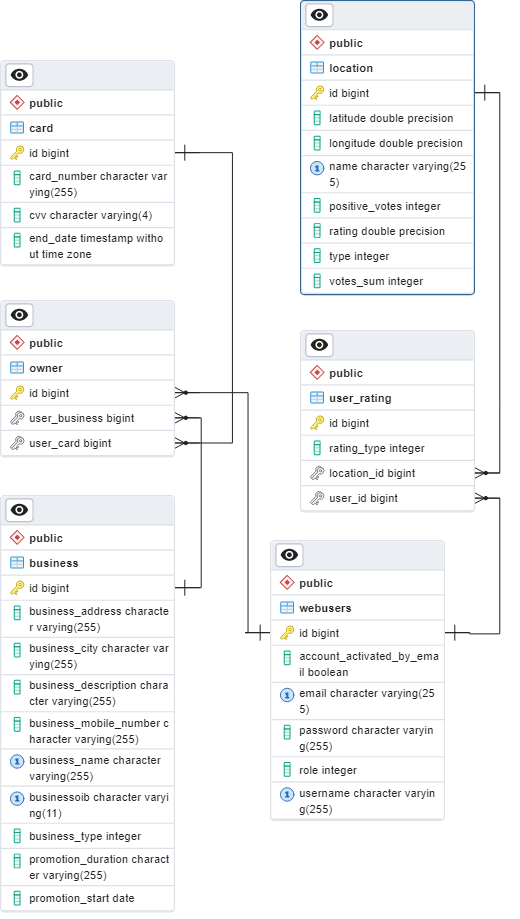
\includegraphics[height=20cm]{slike/ERD.png} %veličina u odnosu na širinu linije
			    \caption{Dijagram baze podataka}
			    \label{fig:ERD} %label mora biti drugaciji za svaku sliku
		    \end{figure}
			
		\pagebreak
		\section{Dijagram razreda}
            Na slikama 4.2-4.7 nalaze se dijagrami razreda koji pripadaju web aplikaciji.
            \\
            
		    \begin{figure}[H]
			    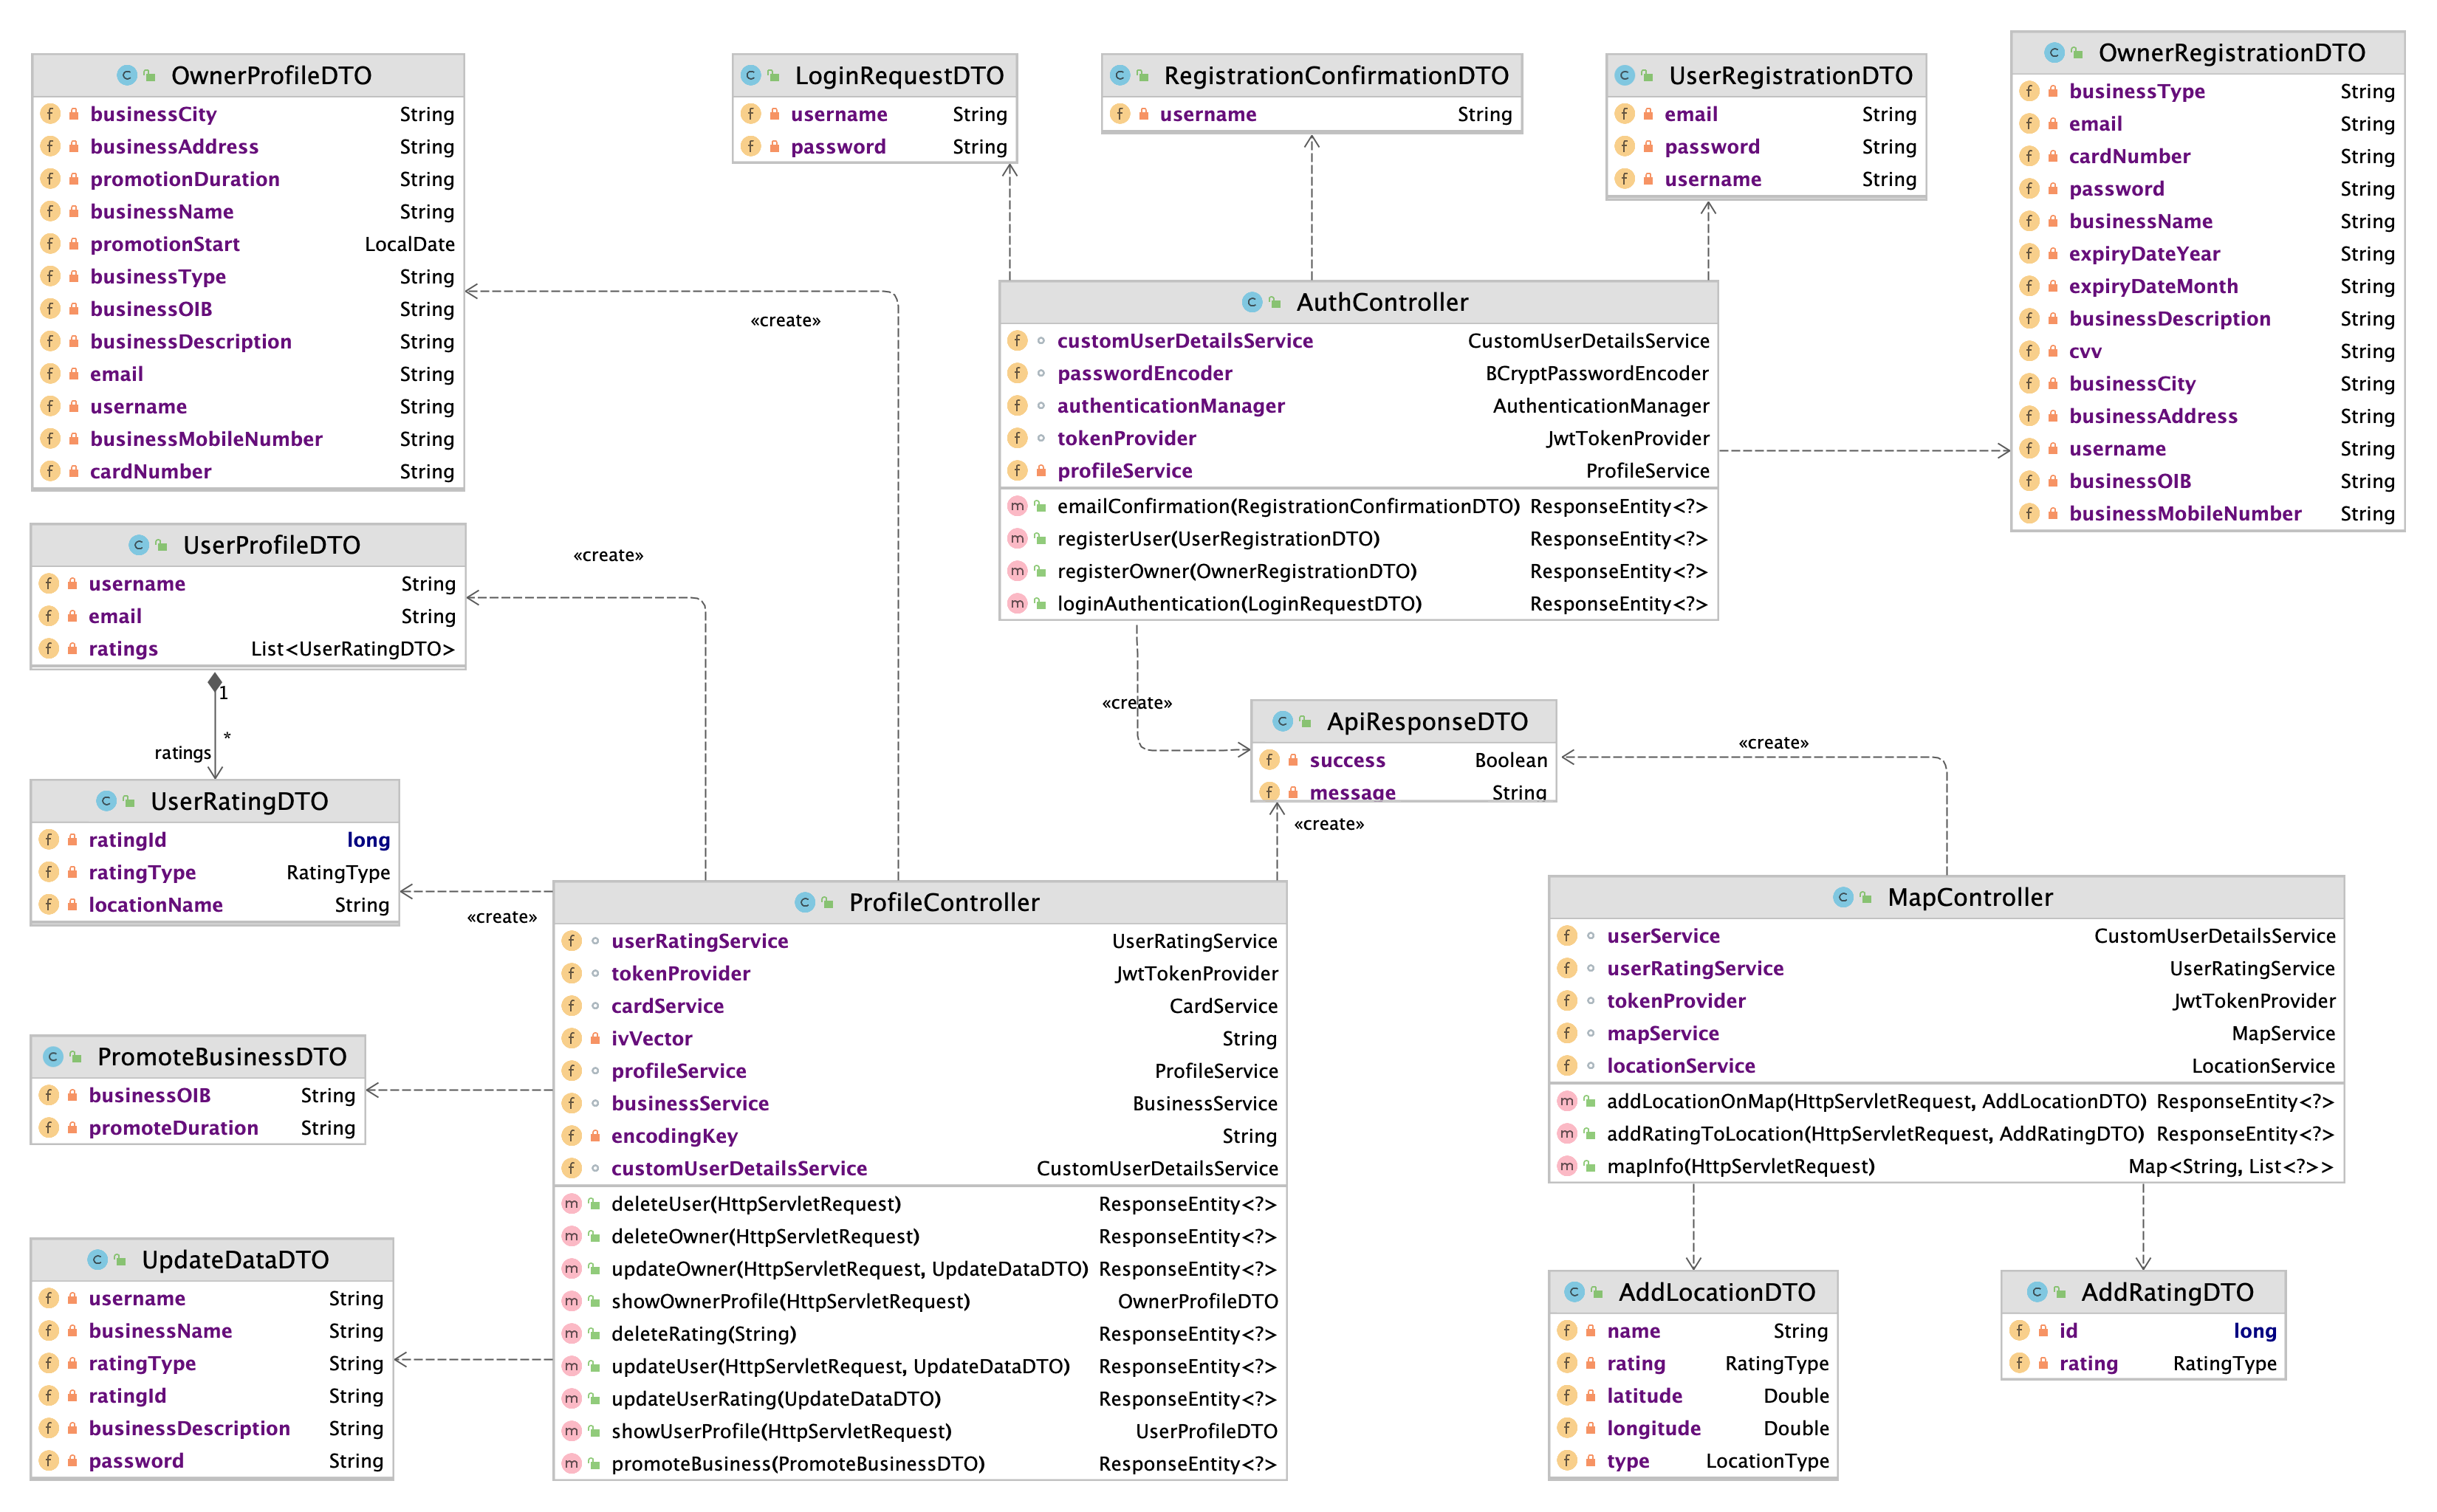
\includegraphics[width=\textwidth]{slike/DR-dto-controller.png} %veličina u odnosu na širinu linije
			    \caption{Dijagram klasa i metoda - Objekti za slanje podataka i controlleri}
                {\small Prikazuje pomoćne DTO (Data Transfer Object) klase koje služe kao okvir unutar kojega se mogu slati zahtjevi i odgovori na zahtjeve. Primjerice, za zahtjeve možemo vidjeti da razred AuthController prima LoginRequestDTO. S druge strane, za odgovore možemo vidjeti da razrede UserProfileDTO i OwnerProfileDTO stvara ProfileController.}
			    \label{fig:DTO} %label mora biti drugaciji za svaku sliku
		    \end{figure}
            \\

            \begin{figure}[H]
                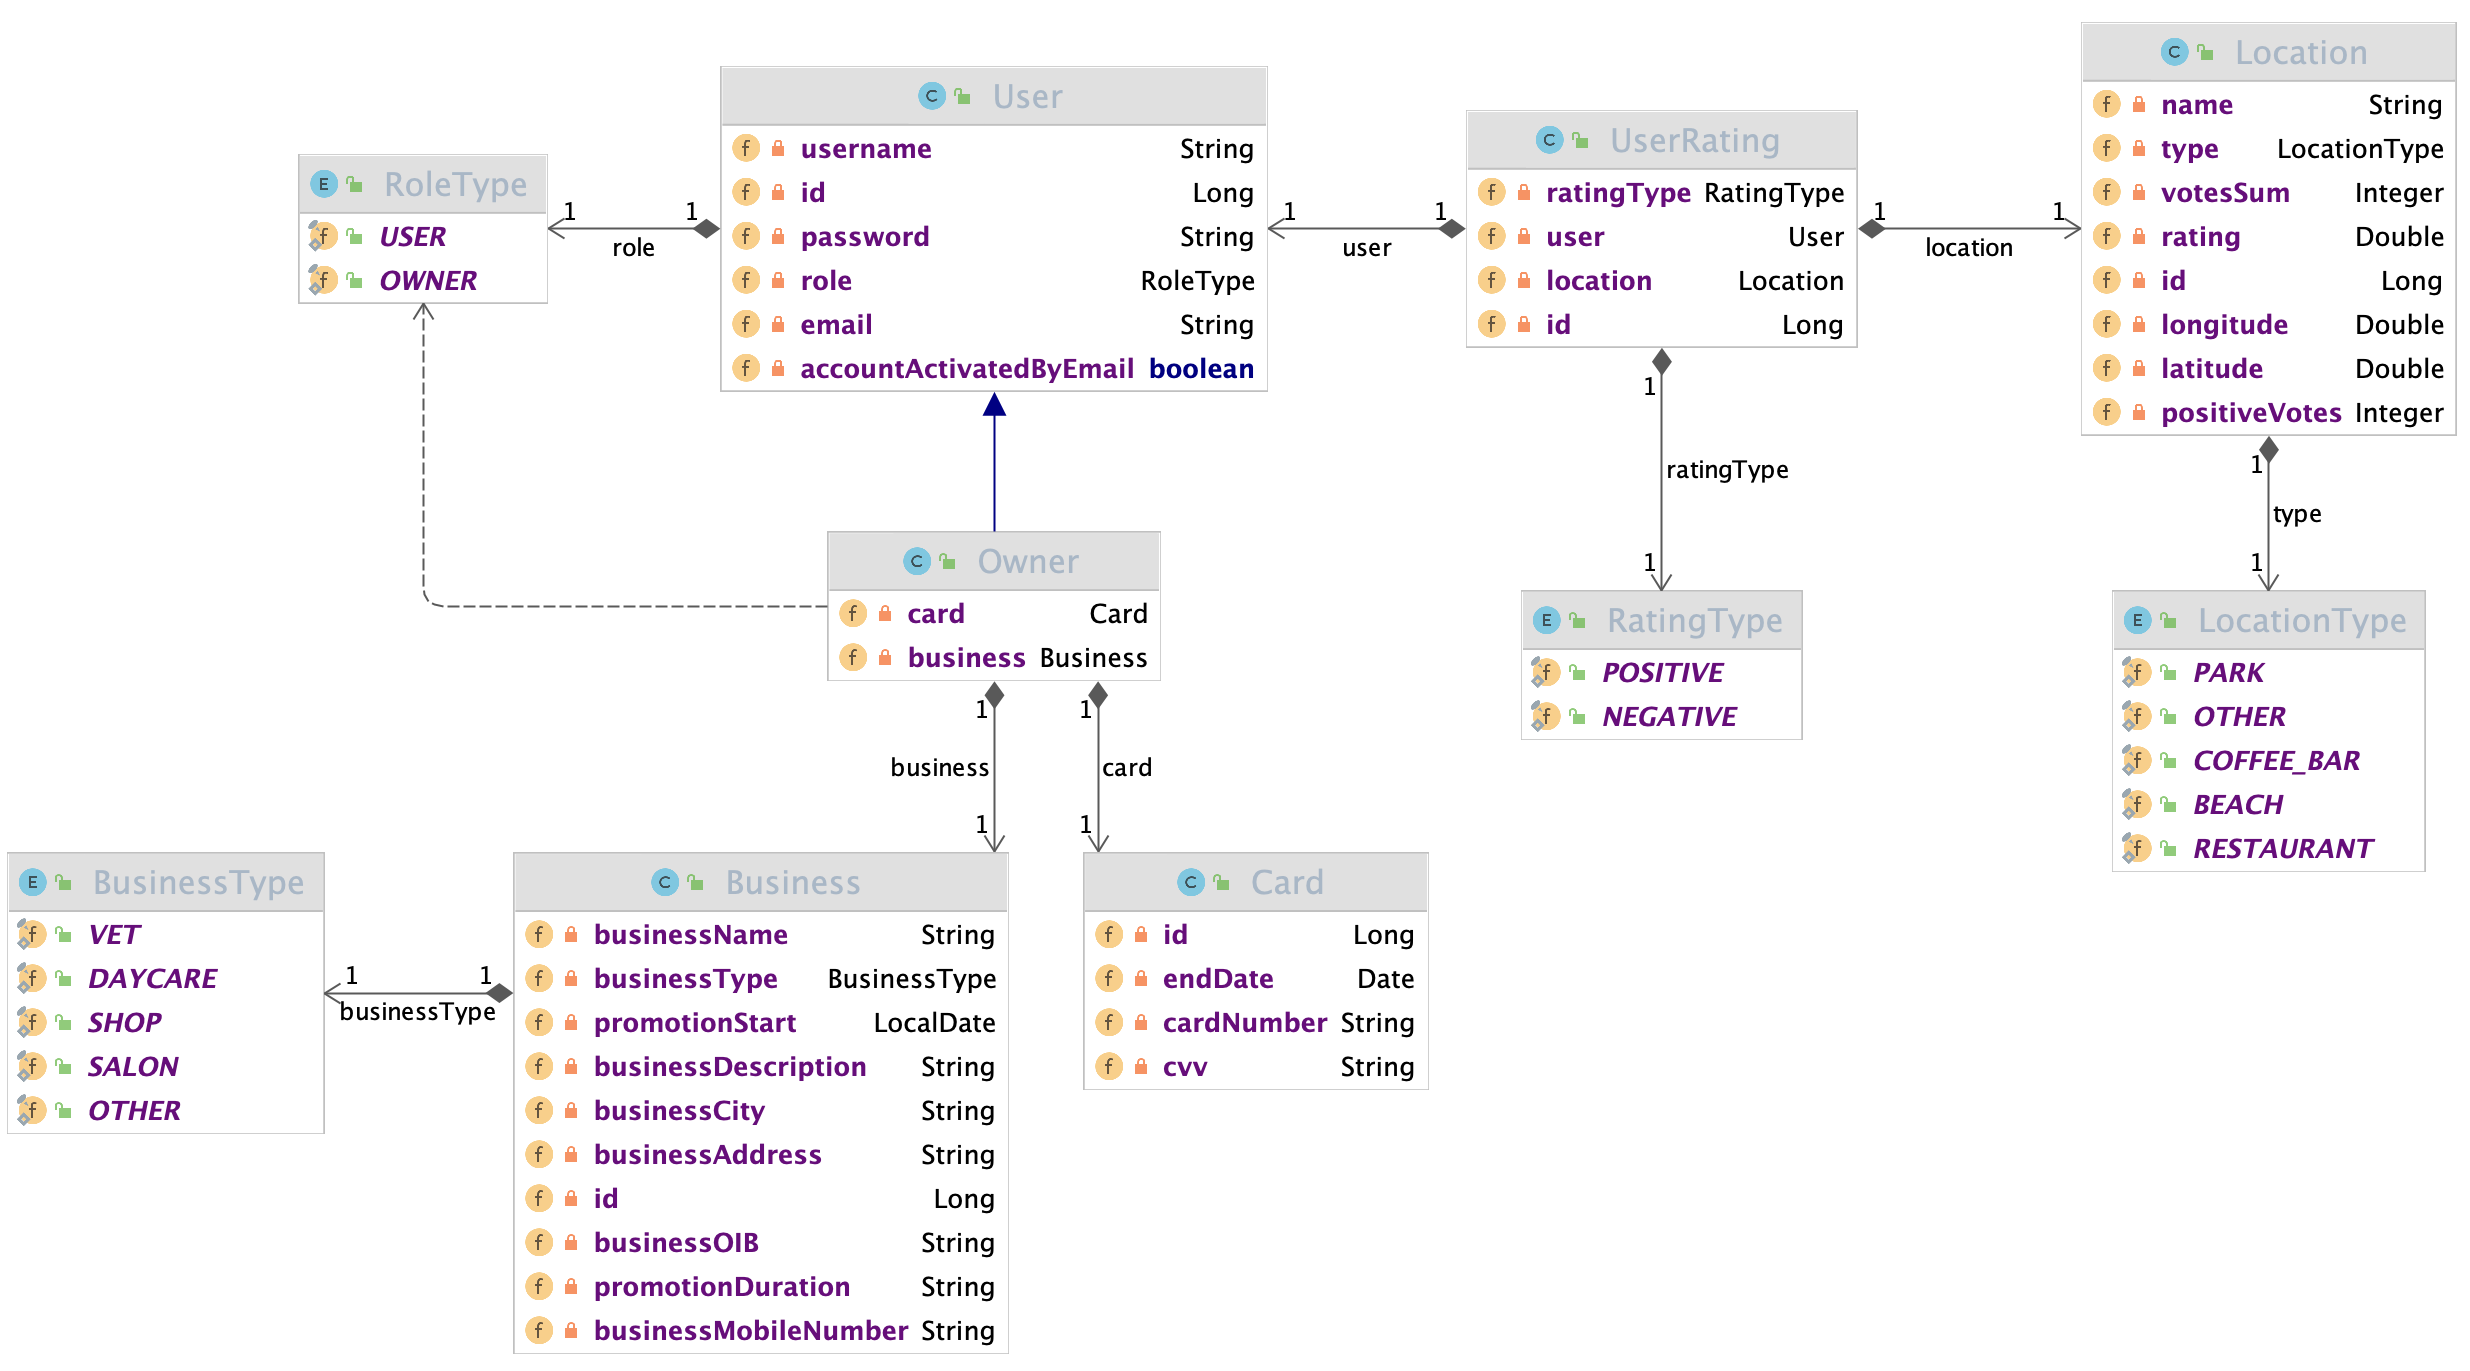
\includegraphics[width=\textwidth]{slike/DR-entities.png} %veličina u odnosu na širinu linije
                \caption{Dijagram klasa i metoda - Objekti i enumeracije}
                {\small Prikazuje razrede koji reprezentiraju objekte koji se spremaju u bazu podataka te sudjeluju kao aktori u aplikaciji te enumeracije koje koristimo kao atribute prikazanih entiteta.}
                \label{fig:OBJ} %label mora biti drugaciji za svaku sliku
            \end{figure}
            \\

            \begin{figure}[H]
                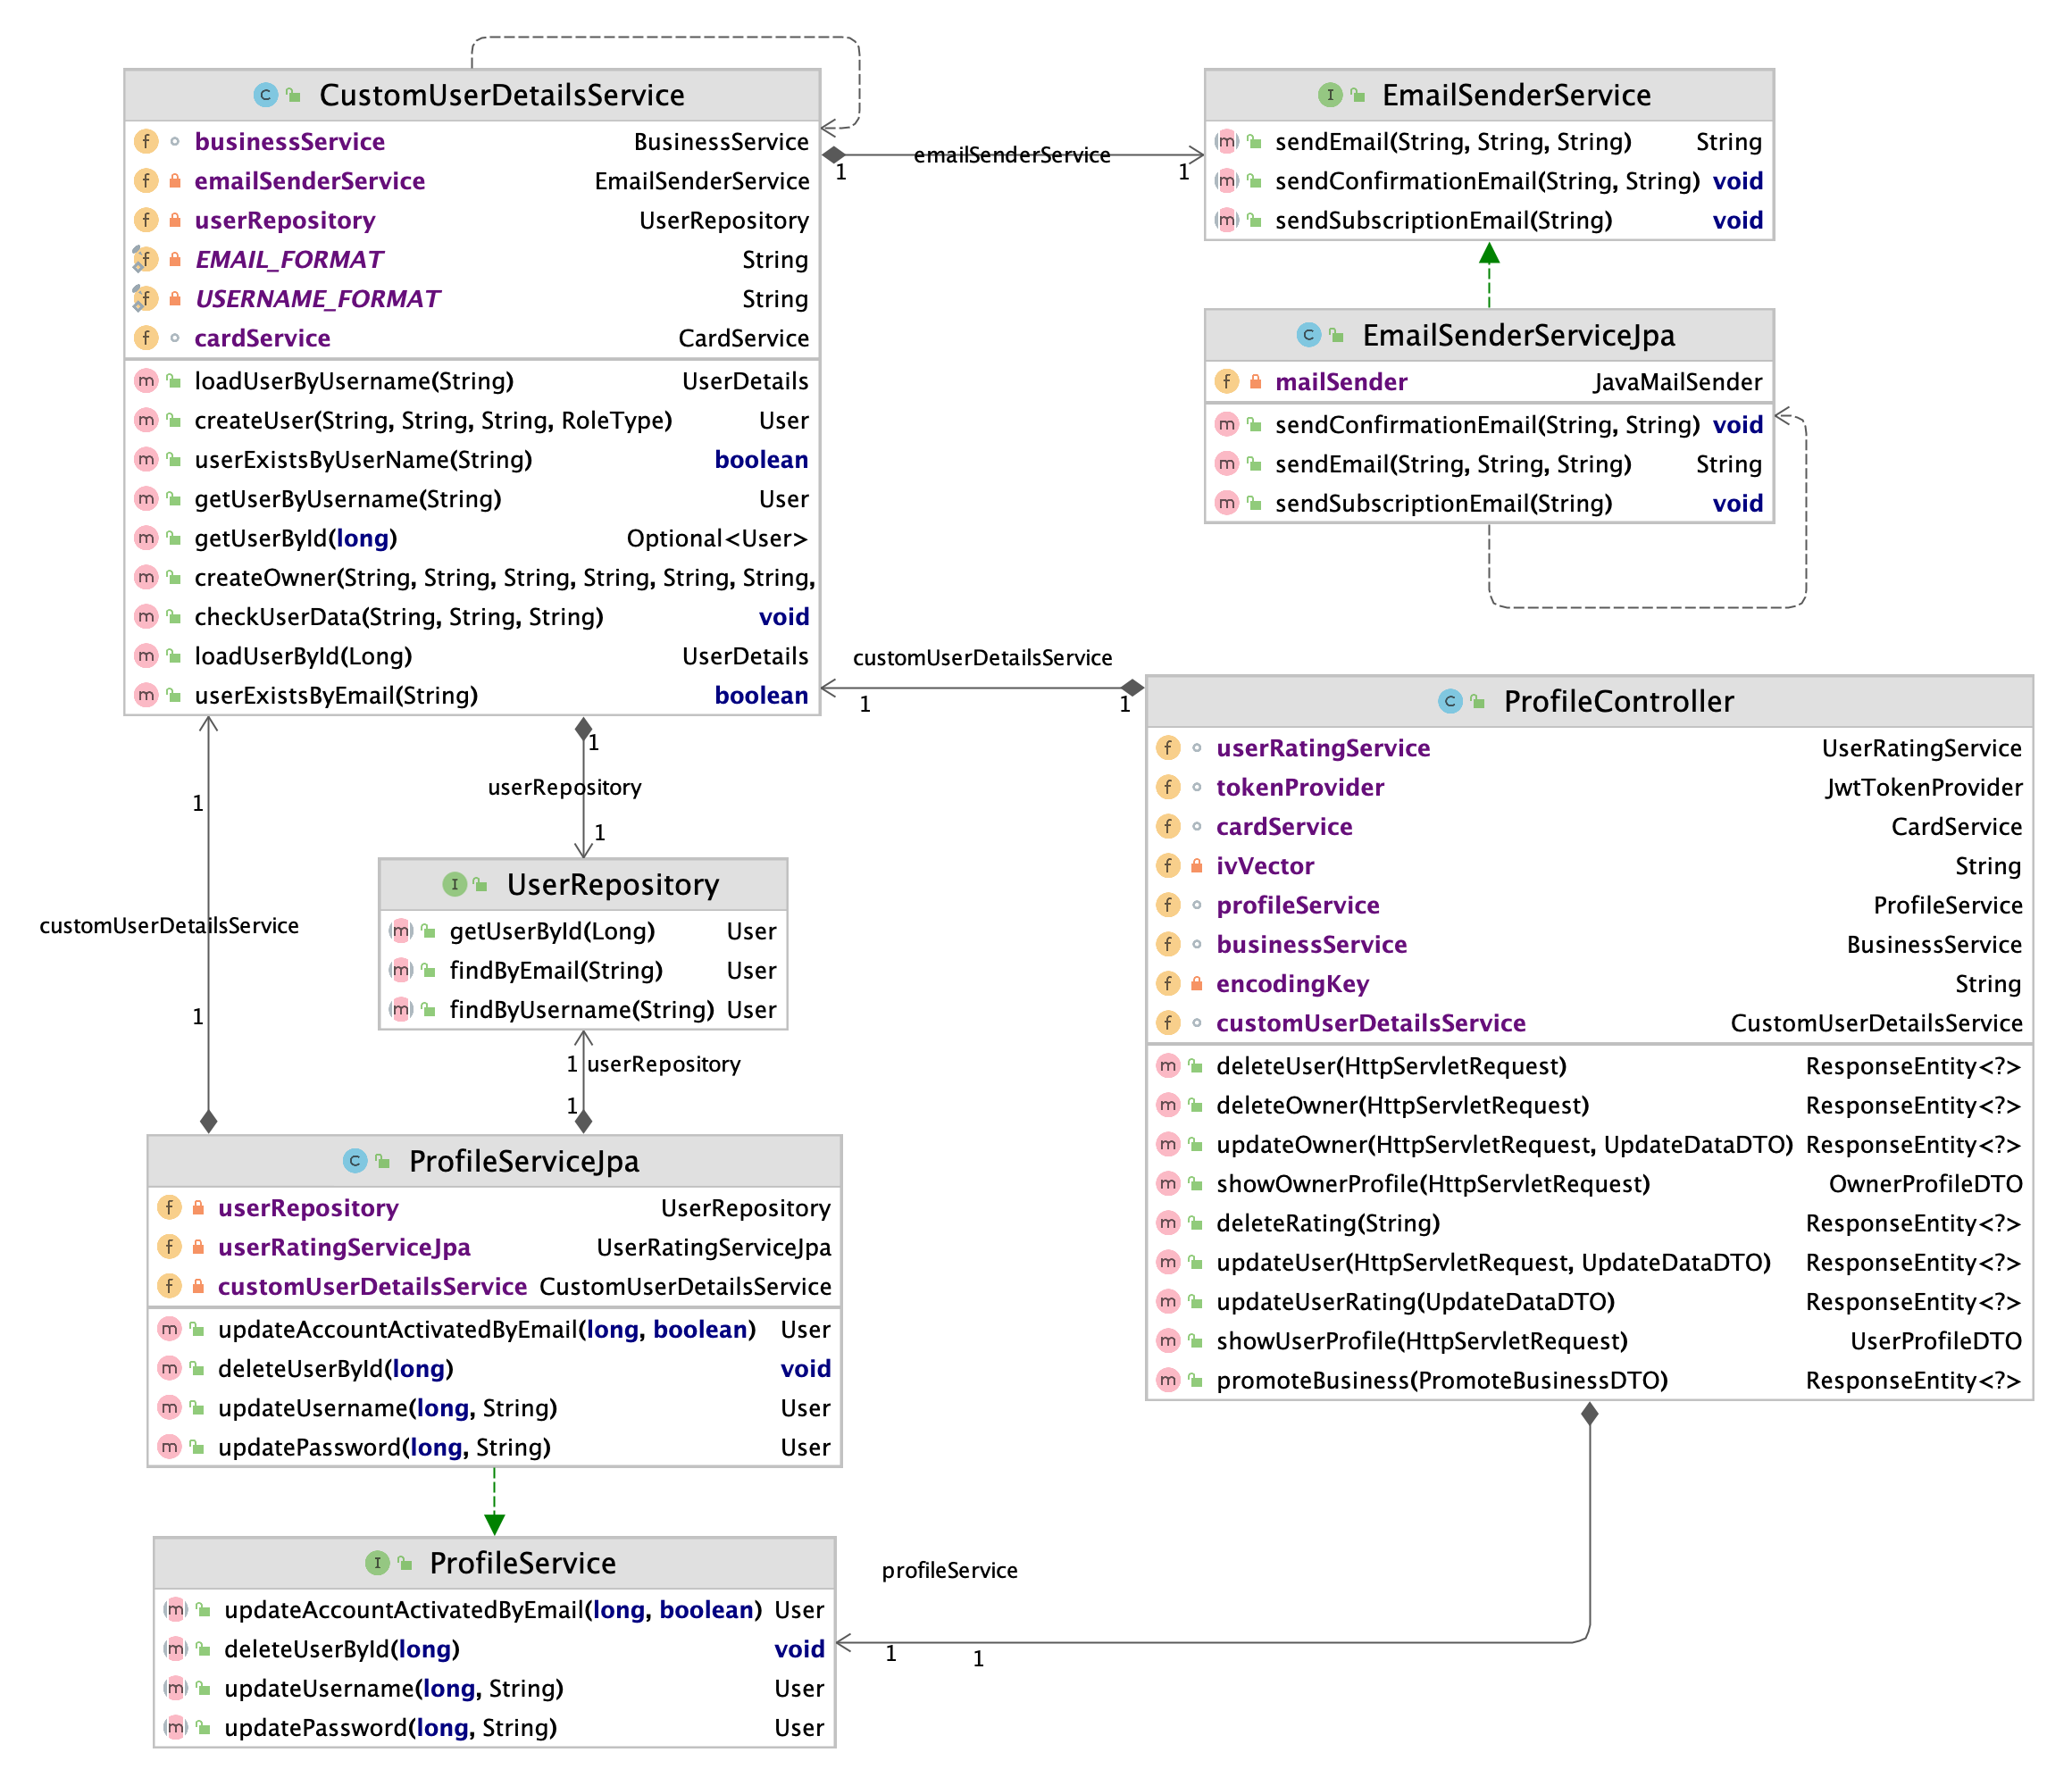
\includegraphics[width=\textwidth]{slike/DR-users.png} %veličina u odnosu na širinu linije
                \caption{Dijagram klasa i metoda - Korisnici}
                {\small Prikazuje strukturu razreda vezanih uz korisnika. CustomUserDetailsService je razred koji koristimo prilikom registracije i prijave korisnika. ProfileController preuzima zahtijeve na profilu korisnika i prosljeđuje zadatke ProfileService-u. Podacima se pristupa putem UserRepository-a. Dodatno je prikazan i EmailSenderService zadužen za slanje e-maila prilikom registracije korisnika.}
                \label{fig:CSR_User} %label mora biti drugaciji za svaku sliku
            \end{figure}
            \\

            \begin{figure}[H]
                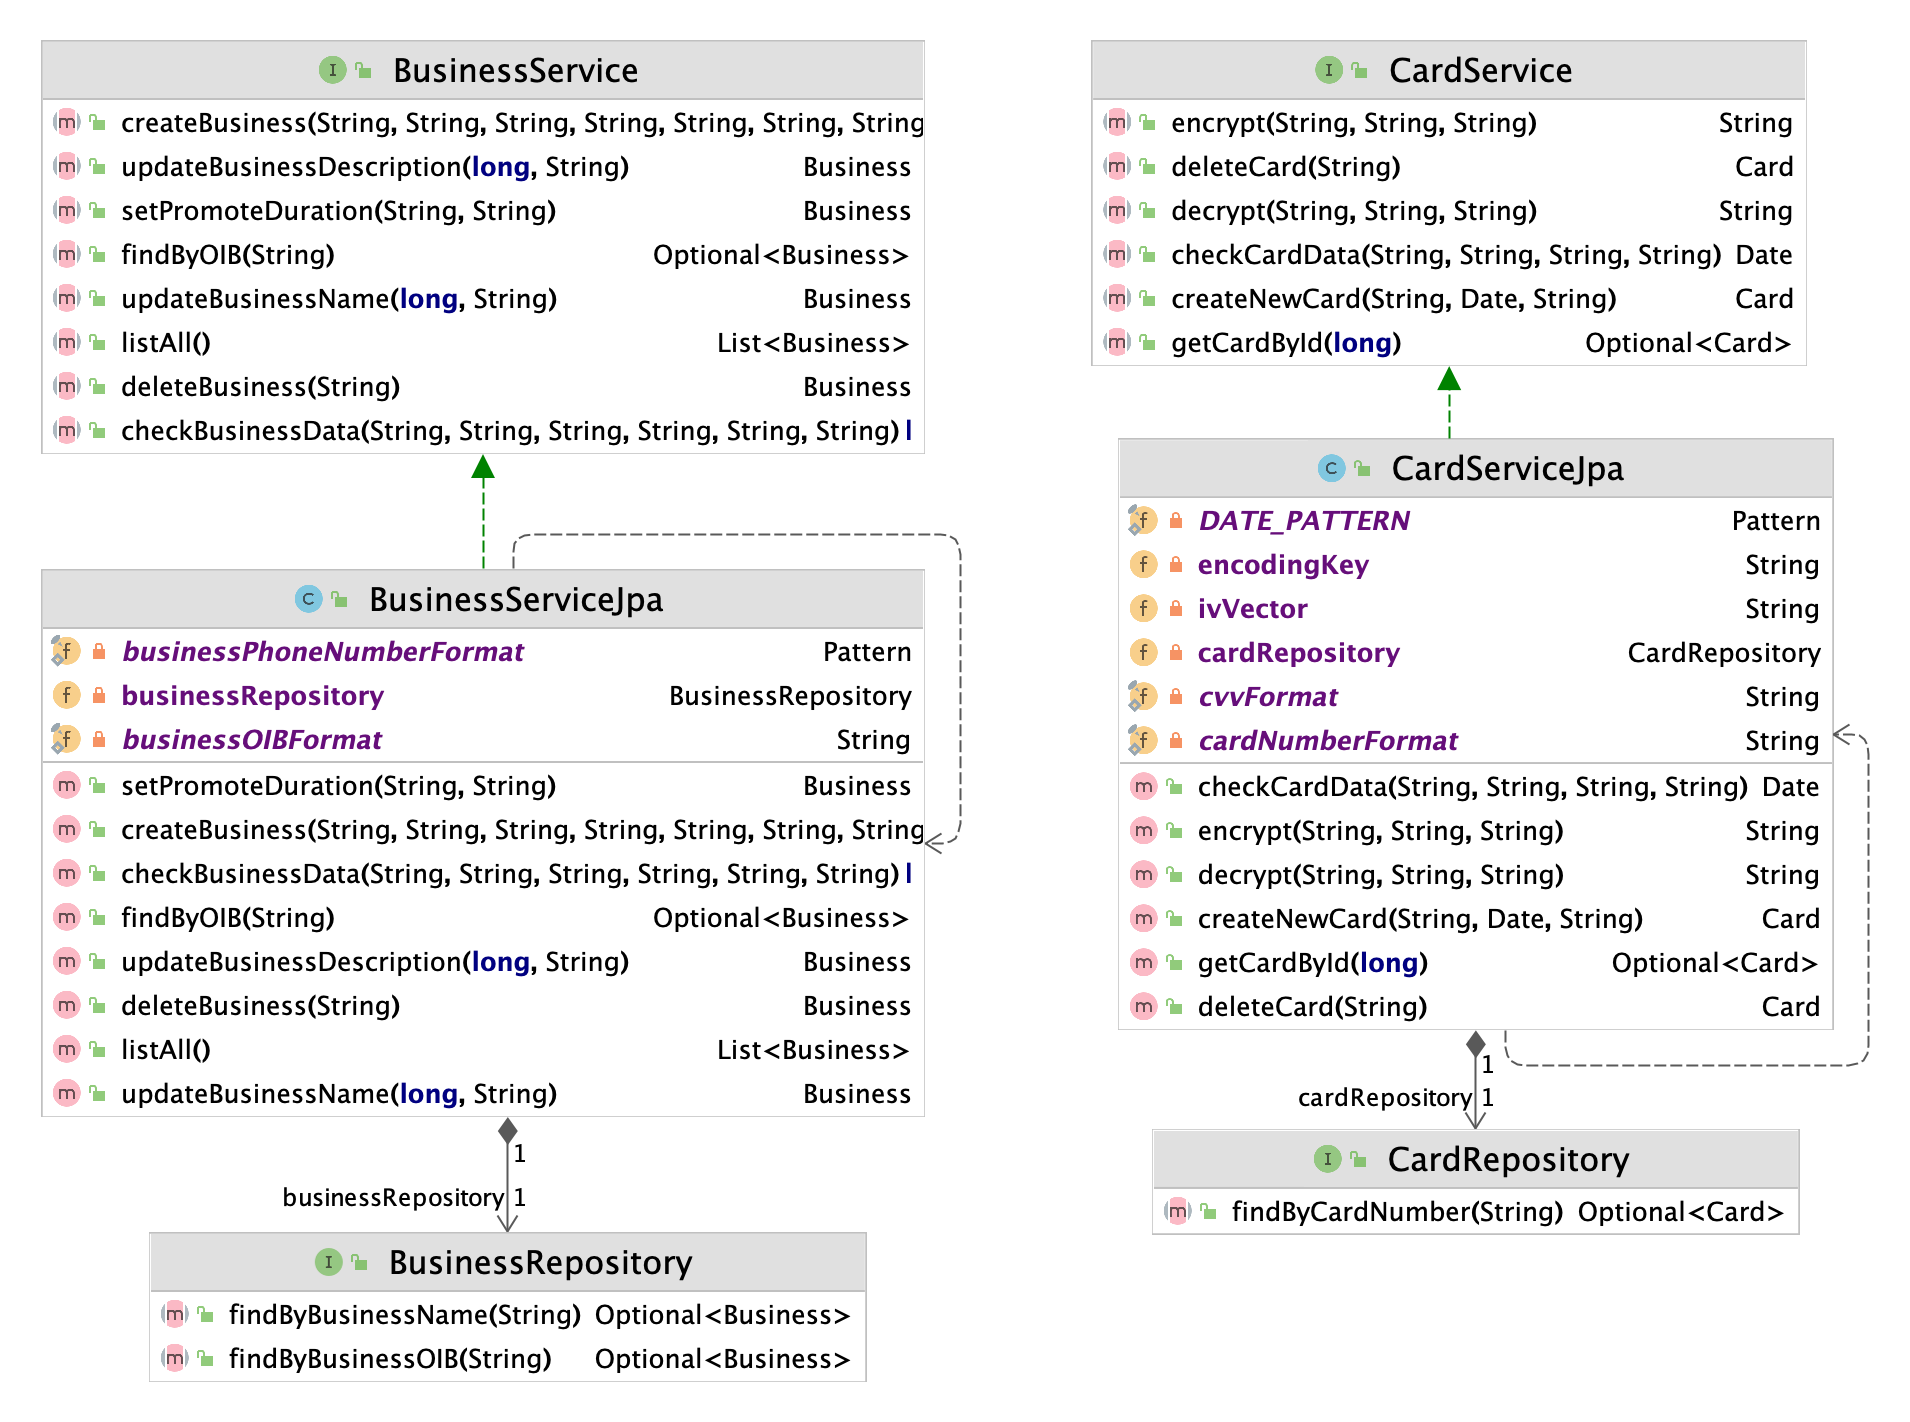
\includegraphics[width=\textwidth]{slike/DR-business-card.png} %veličina u odnosu na širinu linije
                \caption{Dijagram klasa i metoda - Obrt i kartica}
                \centerline{\small Prikazuje Service i Repository sloj za entitete Business i Card.}
                \label{fig:CSR_Other} %label mora biti drugaciji za svaku sliku
		    \end{figure}
            \\
            
            \begin{figure}[H]
                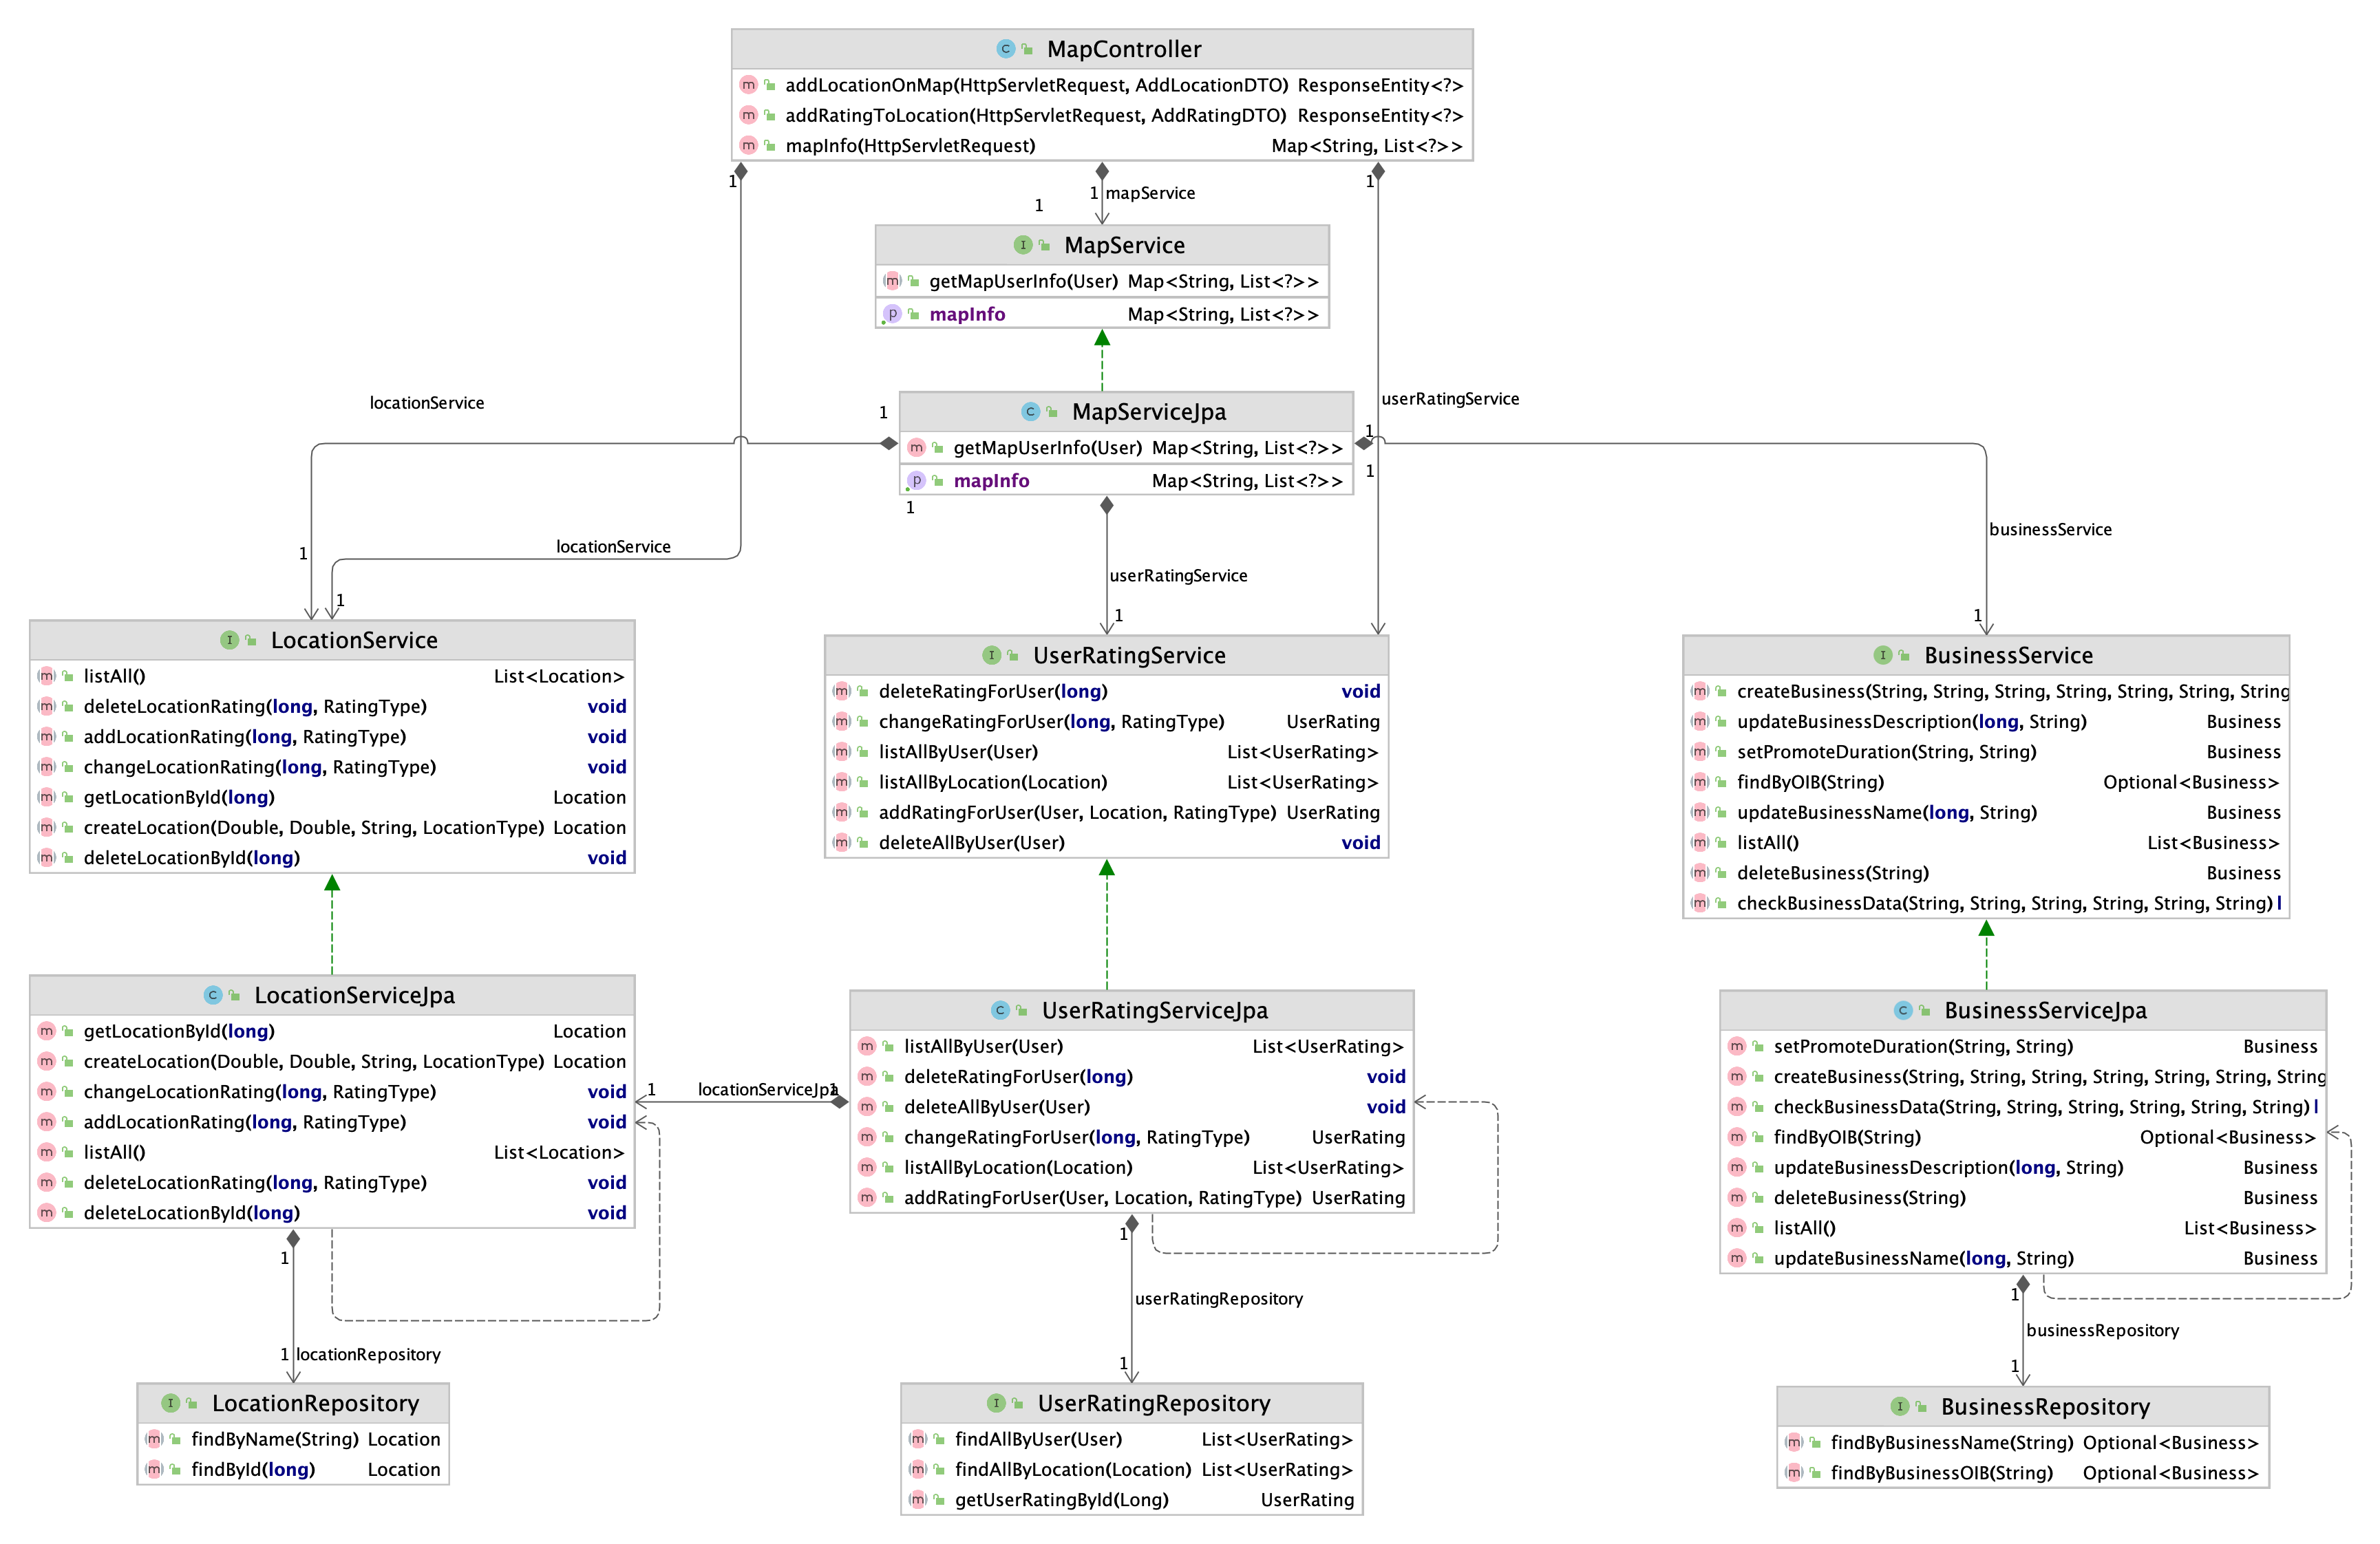
\includegraphics[width=\textwidth]{slike/DR-map.png} %veličina u odnosu na širinu linije
                \caption{Dijagram klasa i metoda - Mapa}
                {\small Prikazuje Controller - Service - Repository model mape, odnosno sve vezano uz obrte, lokacije i ocjene korisnika.}
                \label{fig:CSR_Other} %label mora biti drugaciji za svaku sliku
		    \end{figure}
            \\

            \begin{figure}[H]
                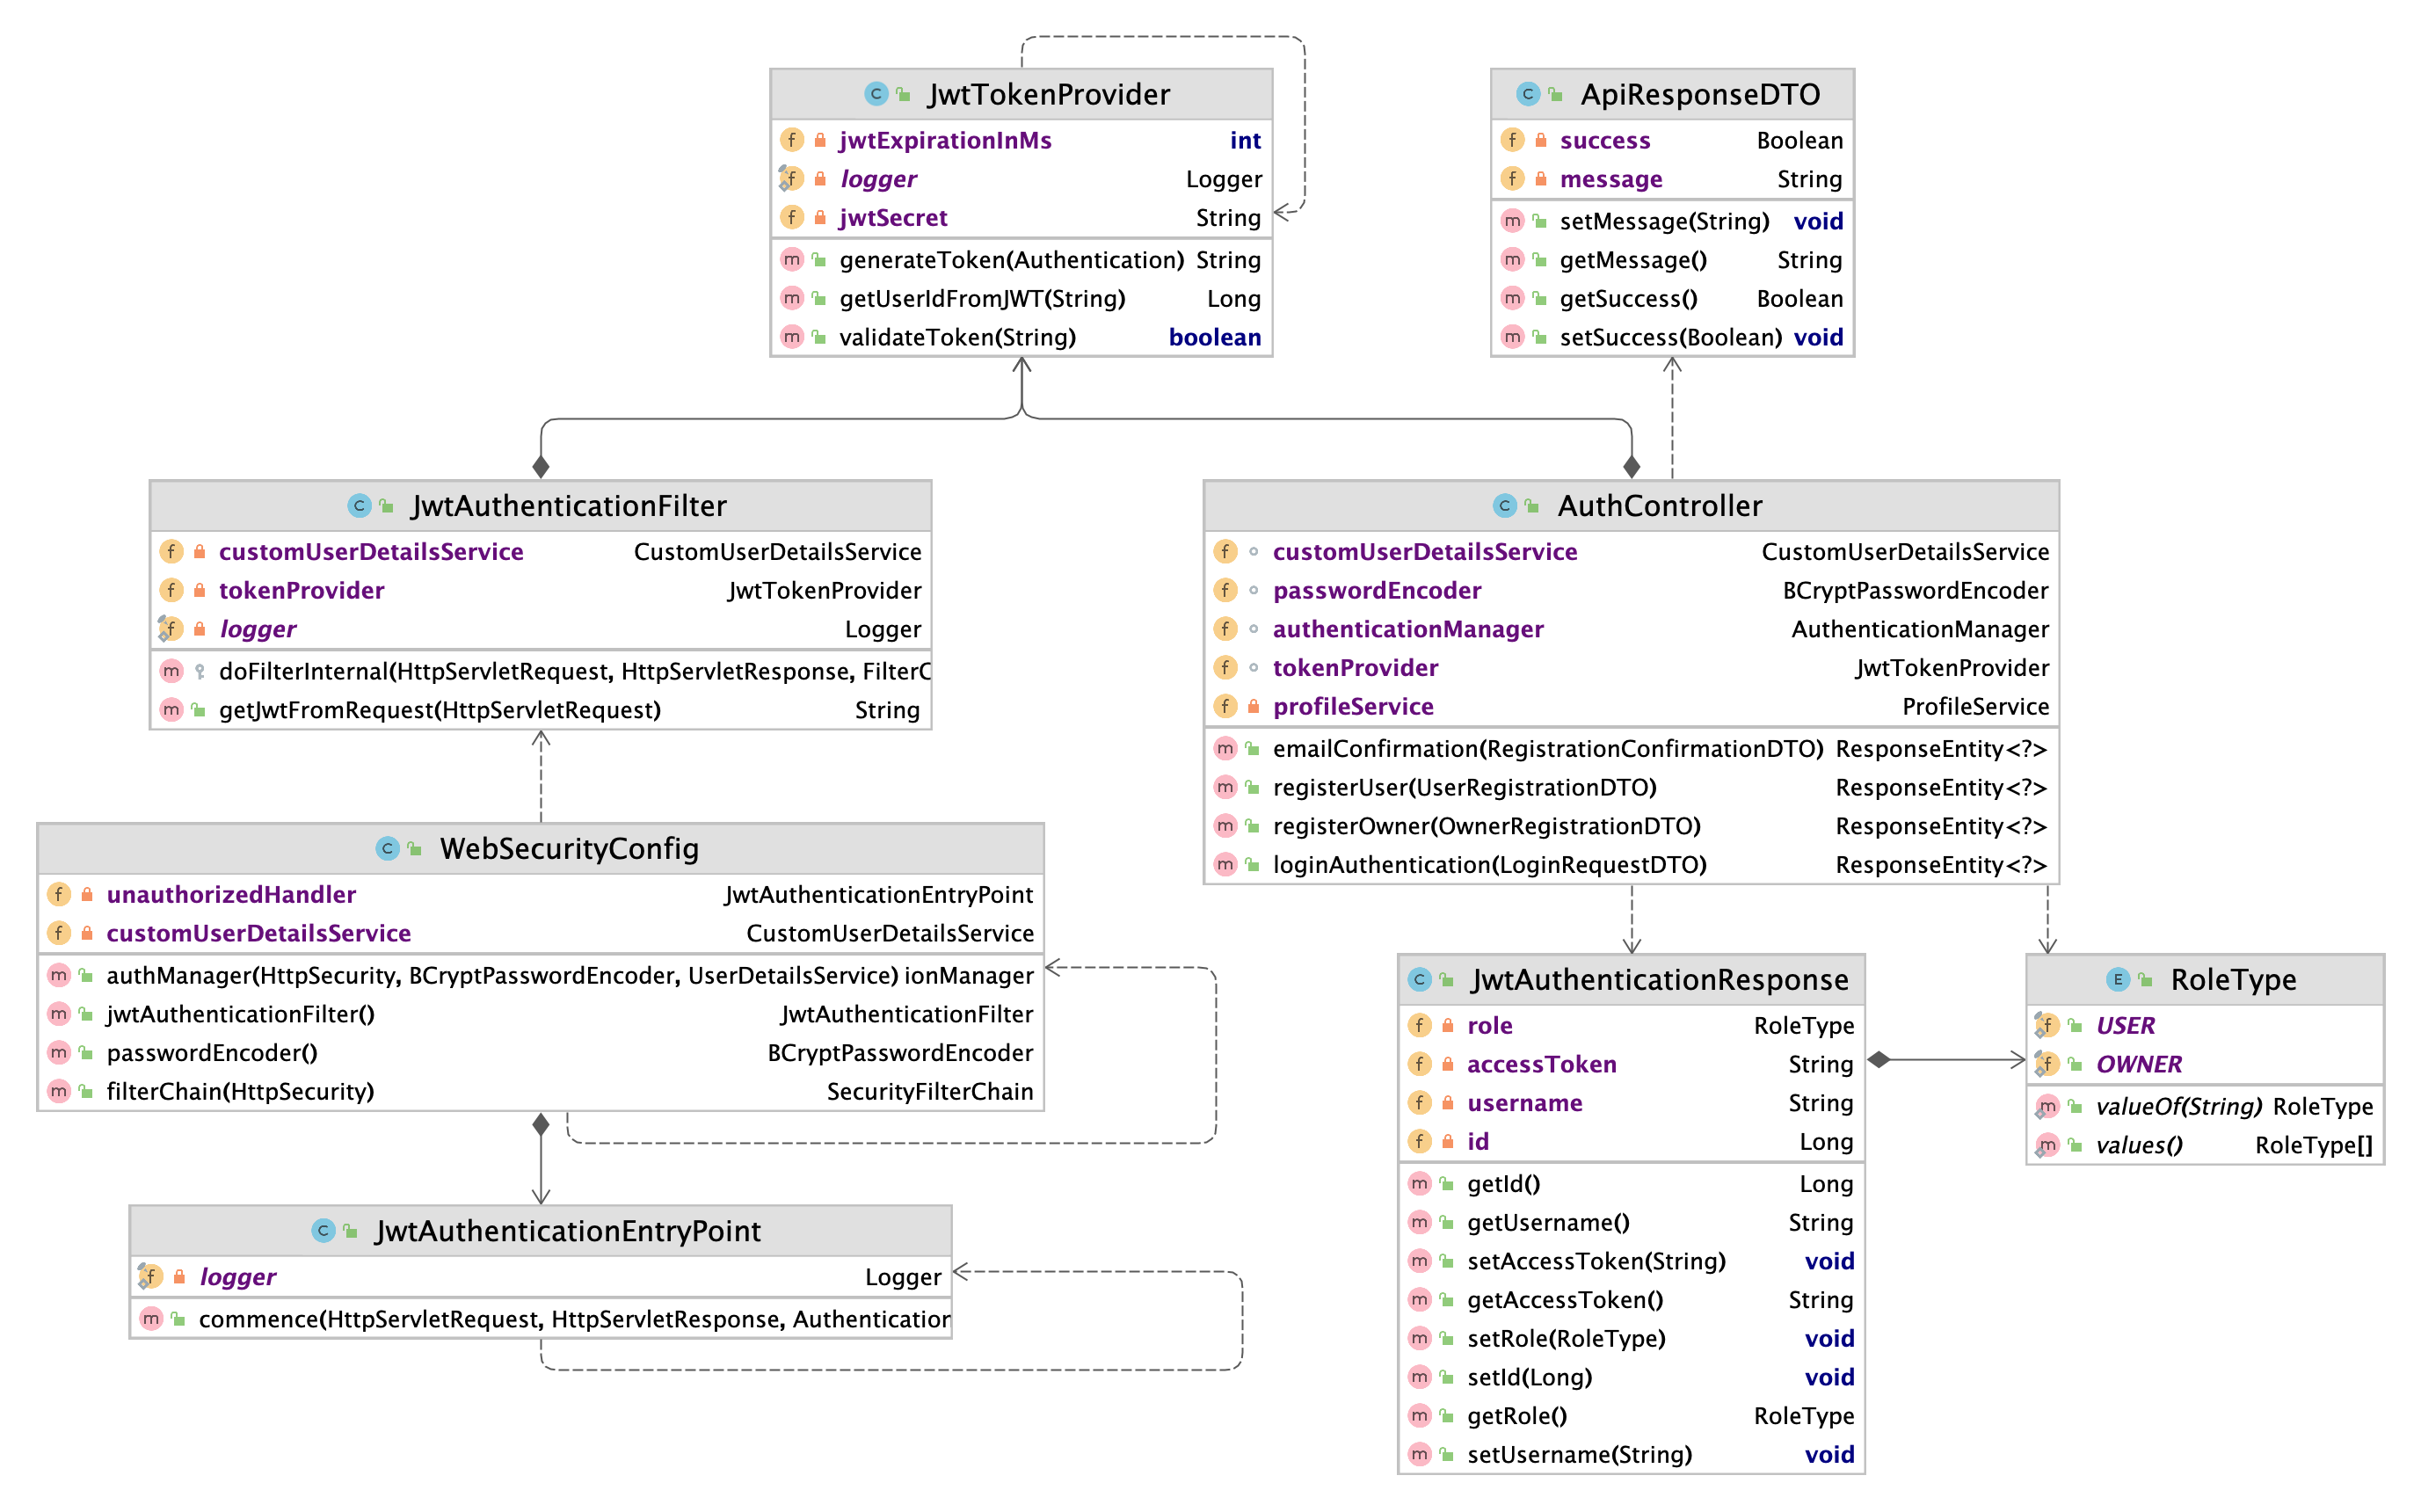
\includegraphics[width=\textwidth]{slike/DR-security.png} %veličina u odnosu na širinu linije
                \caption{Dijagram klasa i metoda - Sigurnost}
                {\small Prikazuje razrede kojima postižemo sigurnost aplikacije. Svi razredi koji započinju s Jwt zaduženi su za ispravno funkcioniranje JSON Web Token sustava. AuthController prima zahtijeve vezane za registraciju i prijavu. WebSecurityConfig je općenita konfiguracija sigurnosti, primjerice autorizacije pristupa određenim URL-ovima.}
                \label{fig:Security} %label mora biti drugaciji za svaku sliku
		    \end{figure}
		
        \newpage
		\section{Dijagram stanja}
			Dijagram stanja prikazuje stanja objekta te prijelaze iz jednog stanja u drugo temeljene
            na dogadajima. Na slici \ref{fig:Dijagram stanja za vlasnika obrta} prikazan je dijagram stanja za vlasnika obrta. Nakon prijave, vlasniku se prikazuje početna stranica, s koje može preći na stranicu karta.
            Na karti može dopustiti pristup vlastitoj lokaciji koja ga centrira, može filtrirati lokacije, te pronaći bilo
            koju važeću lokaciju upisom u tražilicu nakon koje se karta centrira na tu lokaciju.
            Klikom na "Profil" ima opciju promocije vlastitog obrta za koju mora potvrditi plaćanje,
            uređivanja podataka o profilu i obrtu, te brisanje profila.

            \begin{figure}[H]
			    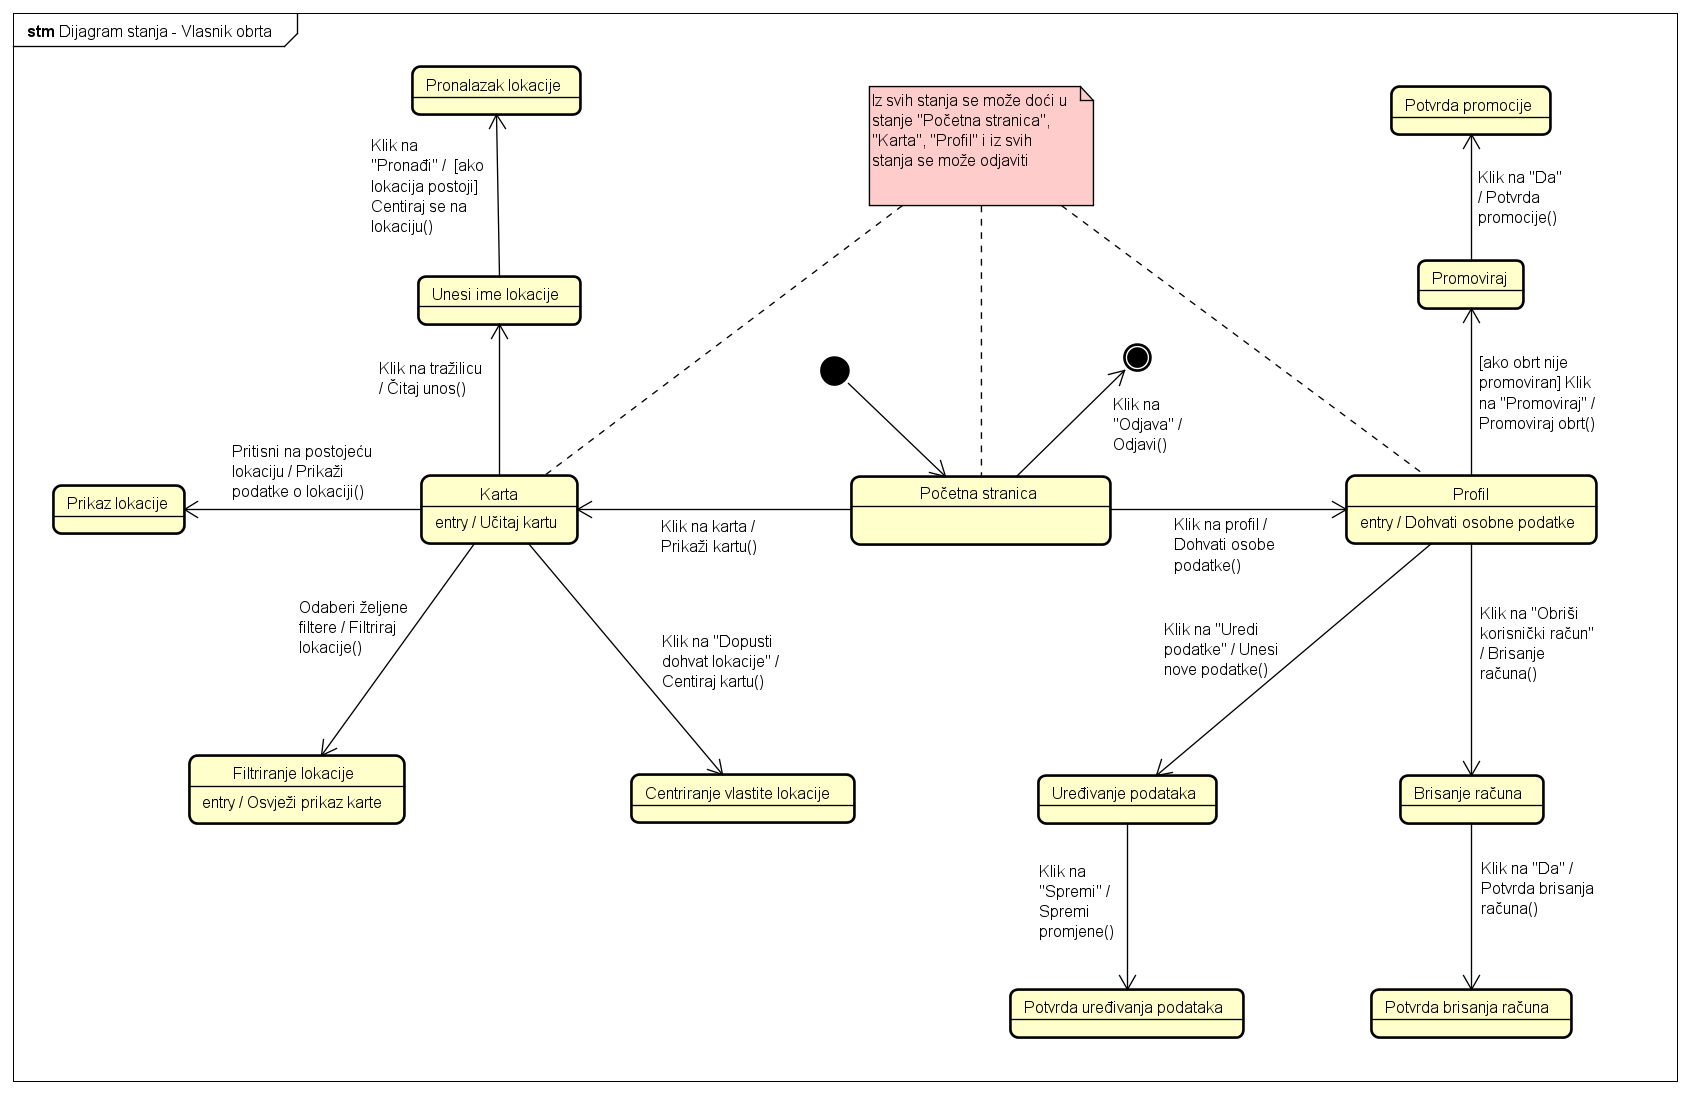
\includegraphics[width=\textwidth]{slike/Dijagram stanja - Vlasnik obrta.png} 
			        \caption{Dijagram stanja za vlasnika obrta}
			    \label{fig:Dijagram stanja za vlasnika obrta}
		    \end{figure}
			
		\newpage
		\section{Dijagram aktivnosti}
            Dijagram aktivnosti služi za modeliranje ponašanja nizom akcija u kojima mogu biti definirani odgovarajući uvjeti prije i nakon izvođenja. Jedna aktivnost obuhvaća više čvorova i veza koji predstavljaju odgovarajući slijed zadataka. Na slici \ref{fig:Dijagram aktivnosti za dodavanje lokacije} prikazan je proces dodavanja lokacije. Korisnik da bi dodao novu lokaciju mora se prvo prijaviti u sustav. Nakon što se prijavio, korisnik mora otići na stranicu Karta gdje može prizvoljno kliknuti na kartu i dodati tu novu lokaciju. Zatim mu se otvara forma za upis gdje joj upisuje željene podatke. Ako su svi podaci ispravni, karta se centrira na novododanu lokaciju.
            
            \begin{figure}[H]
			    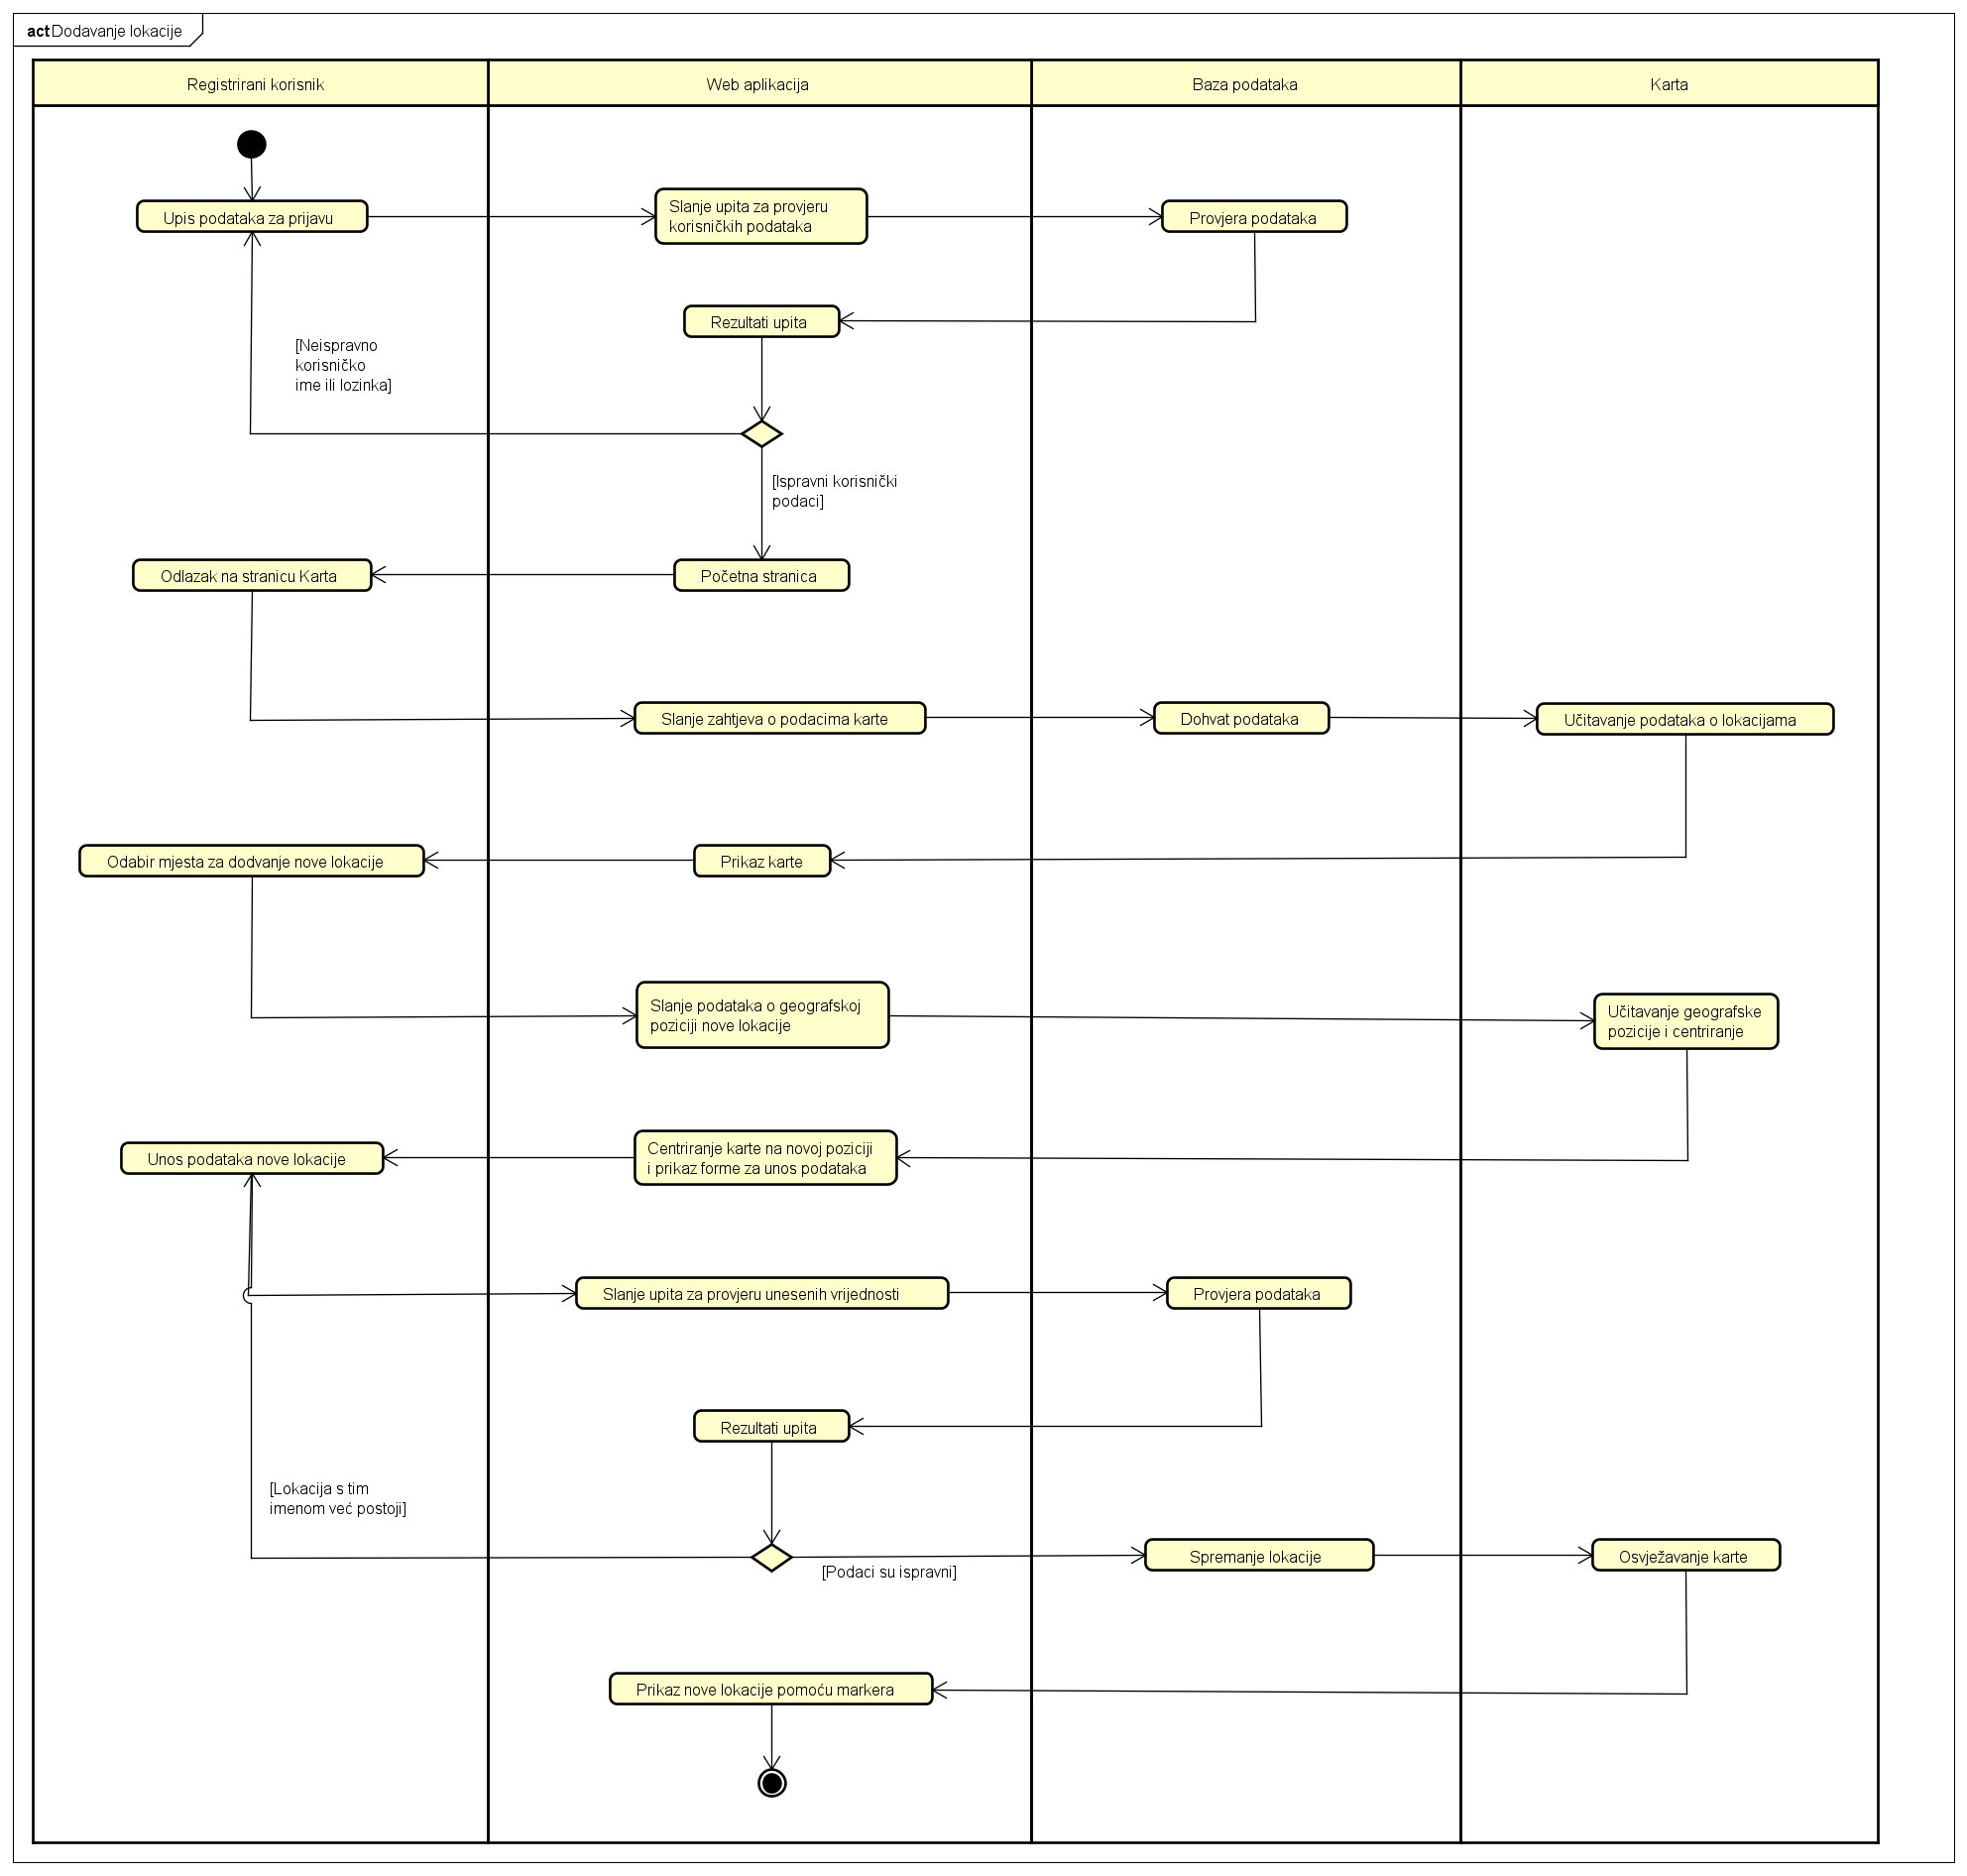
\includegraphics[width=\textwidth]{slike/Dijagram aktivnosti - Dodavanje lokacije.png} 
			        \caption{Dijagram aktivnosti za dodavanje lokacije}
			    \label{fig:Dijagram aktivnosti za dodavanje lokacije}
		    \end{figure}
      
		\newpage
		\section{Dijagram komponenti}
		  Dijagram komponenti prikazan na slici \ref{fig:Dijagram komponenti za Dog Friendly aplikaciju} opisuje organizaciju i međuovisnost komponenti, interne strukture i odnose prema okolini. Sustavu se pristupa preko dva različita sučelja. Preko sučelja za dohvat HTML, CSS i JS datoteka poslužuju se datoteke koje pripradaju frontend dijelu aplikacije. Router je komponenta koja na upit s url određuje koja datoteka će se poslužiti na sučelje. Frontend dio se sastoji od niza JavaScript datoteka koje su raspoređene u logičke cjeline nazvane po tipovima aktora koje im pristupaju. Sve JavaScript datoteke ovise o React biblioteci iz koje dohvaćaju gotove komponente kao što su gumbi, forme i slično. Preko sučelja za dohvat JSON podataka pristupa se REST API komponenti. REST API poslužuje podatke koji pripadaju backend dijelu aplikacije. Spring Framework je zadužen za dohvaćanje tablica iz baze podataka pomoću SQL upita. Podaci koji su pristigli iz baze se šalju dalje u arhitekturu Controller-Service-Repository u obliku DTO-a (Data transfer object). React-view komponenta preko dostupnih sučelja komunicira sa Dog Friendly aplikacijom te ovisno o korisnikovim akcijama osvježava prikaz i dohvaća nove podatke ili datoteke.
            
            \begin{figure}[H]
			    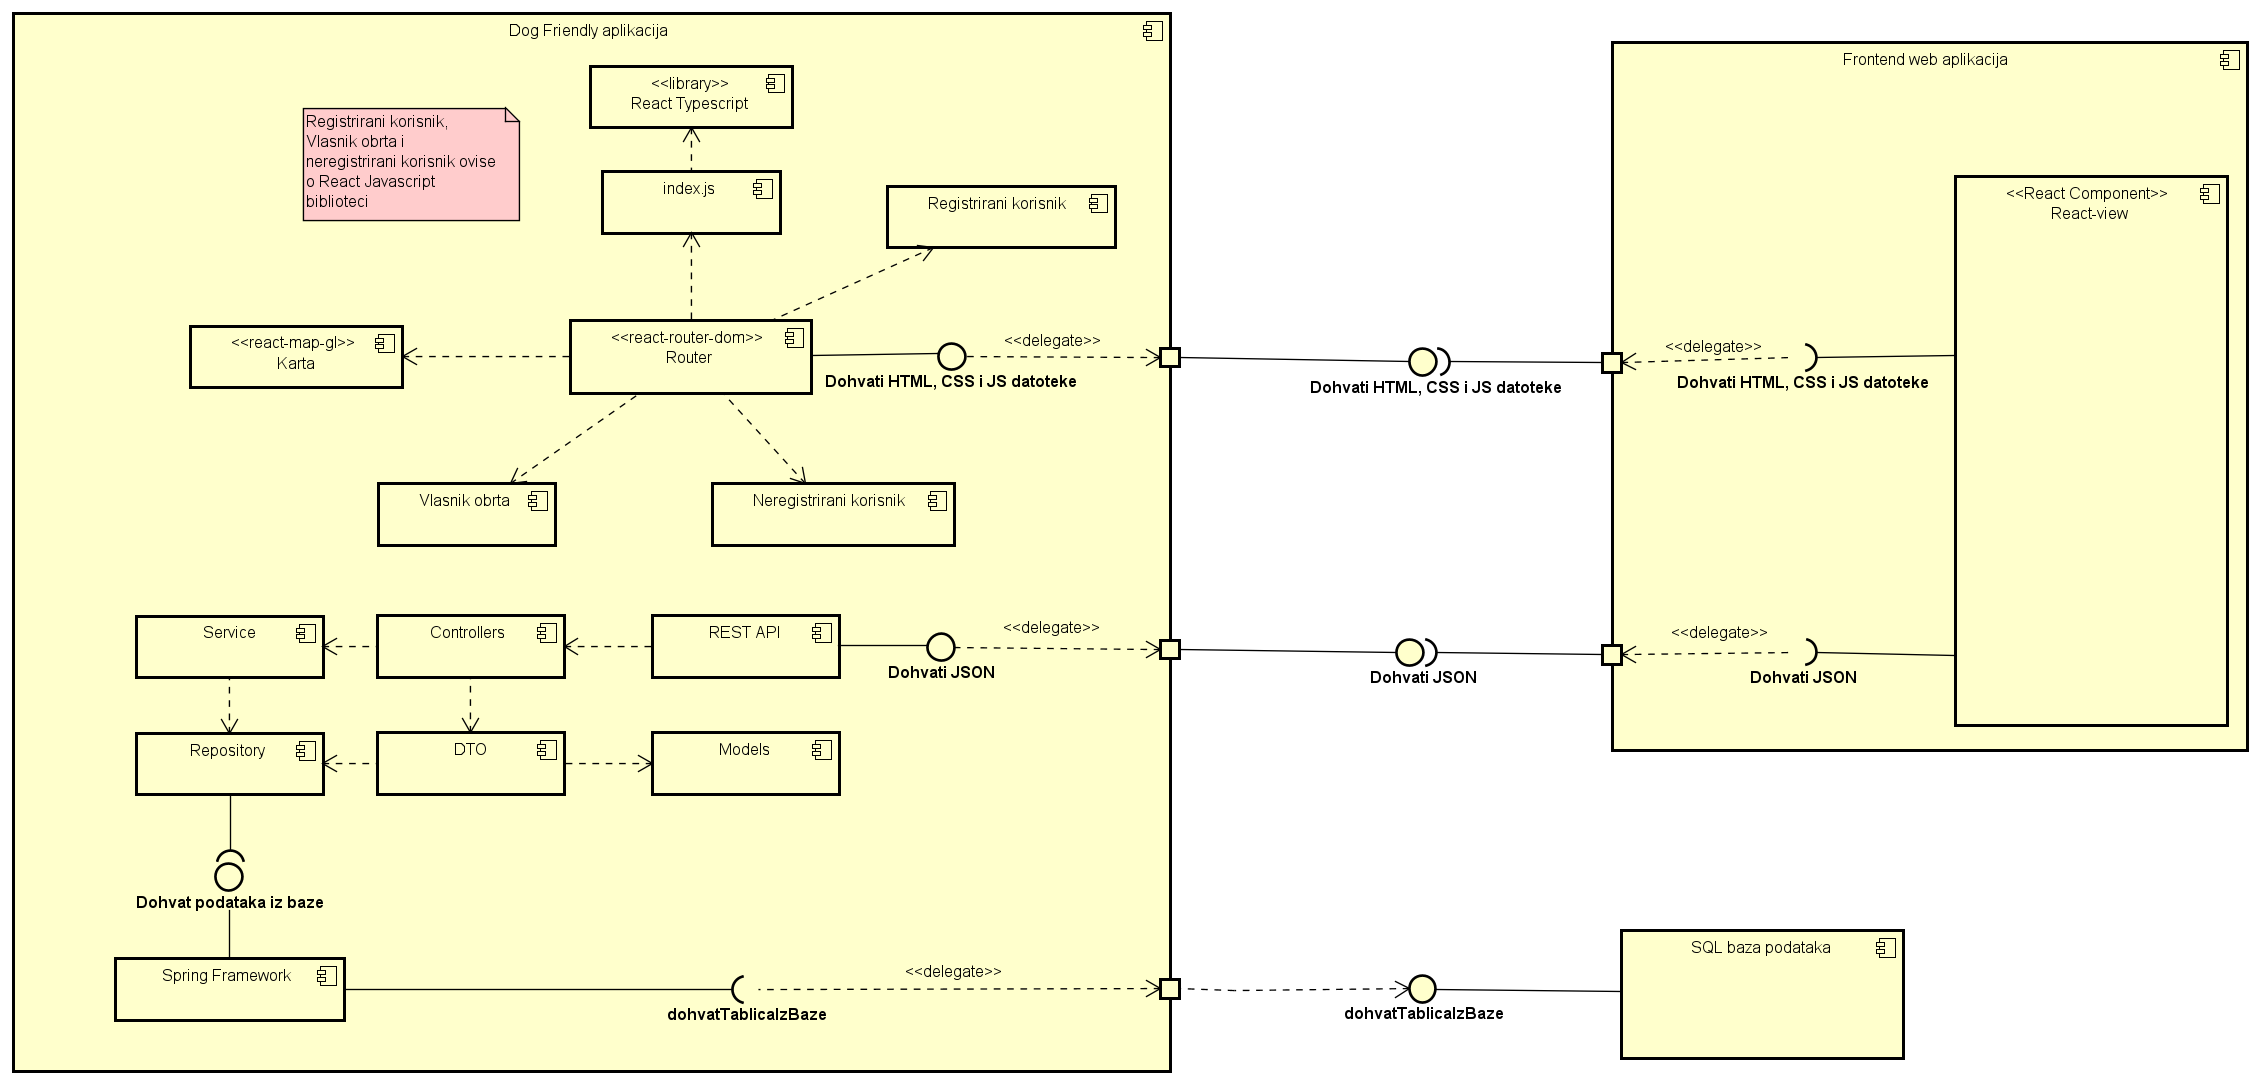
\includegraphics[width=\textwidth]{slike/Dijagram komponenti - Dog Friendly aplikacija.png} 
			        \caption{Dijagram komponenti za Dog Friendly aplikaciju}
			    \label{fig:Dijagram komponenti za Dog Friendly aplikaciju}
		    \end{figure}